% ========================================= TEMPLATE INFO ========================================
%
% Author:       P4ntomime
% Version:      1.0.0
% Last updated: 2024-02-18
% Brief:        A LaTeX template for summaries. See README.md for more information.
% 
% ================================================================================================
\documentclass[8pt, a4paper, twoside, landscape]{extarticle}
% Font size:    8pt
% Paper size:   A4
% style:        twoside (needed, so odd and even pages have different margins)
% orientation:  portrait. (use 'landscape' for landscape orientation)


% ========================================= DOCUMENT INFO =========================================
\def\title{Prog C++}                                        % title
\def\shorttitle{Prog C++}                                   % short title (displayed as PDF title)
\def\dozent{Prof. Dr. Christian Werner}                     % lecturer
\def\semester{FS 2026}                                      % semester
\def\author{Fabian Steiner}                                 % author(s)
\def\contributors{Mirko Ratti}                              % contributor(s) (optional -> comment out if none)
\def\repo{https://github.com/Iceteavanill/Cheatsheet-Prog_Cpp_FS_2024_OST}     % repository link
\def\version{2.0.\today}                                    % version
\def\pagelimit{16}                                          % page limit -> causes pages after limit to be red
\def\titleoption{ultra compact}                             % options: ultra compact, compact, normal
\def\enableToC{false}

% ================================= PACKAGES, SETUP AND COMMANDS ==================================
\input{preamble.tex}


% =========================================== DOCUMENT ============================================
\begin{document}
    \begin{layout}
        \section{Basics}

\subsection{Grundsätzlich}

C++ ist sehr ähnlich zu C. Es gibt aber einige wichtige Änderungen zu C:

\begin{itemize}[itemsep=1pt, parsep=0pt]
    \item zu benutzender Compiler heisst jetzt \texttt{clang++}
    \item Nativen Bool Typ : \textbf{bool}
    \item richtiges Konstanten Schlüsselwort : \textbf{constexpr}
    \item Standartbibliotheken haben kein .h mehr beim Aufrufen
    \item C Standartbibliotheken können weiter verwendet werden, haben aber ein C im Header(stdio.h $\rightarrow$ cstdio)
    \item Char-Literale (z. B. 'A') haben in C++ den Datentyp char (in C war es int)(Brauchen ein const)
    \item Es gibt benannte Namensräume. Wichtigster Namensraum für die STL: \texttt{std}
\end{itemize}

\subsection{Hello world C++}

\lstinputlisting{code/01_basics/hello_World.cpp}

\subsection{Range-based for Loop}\label{forEach}

Range based for Loops laufen automatisch ein Array ab, ohne das zuerst die Grösse ermittelt werden muss. 
Die C for loop syntax wurde etwas erweitert.
Syntax:

\lstinputlisting{code/01_basics/forEach.cpp}

Siehe: Als Array Name wird ein \texttt{Pointer} auf das Array verlangt, nicht auf das erste Element!  
Ein foreach funktioniert \textbf{nicht} mit einem \textbf{Pointerpointer}. 

\subsection{Streams}

Ein Stream repräsentiert einen generischen sequentiellen Datenstrom. Z.b: ein Eingabefeld, Dateien oder Netzwerktraffic.\\
Die wichtigsten Operatoren sind:

\begin{itemize}[itemsep=1pt, parsep=0pt]
    \item \verb|<<| : Inserter $\rightarrow$  Daten einfügen
    \item \verb|>>| :  Extractor $\rightarrow$ Daten herausholen
\end{itemize}

Für Standardklassen sind diese Operatoren bereits definiert.

\subsubsection*{Standardstreams}

\begin{itemize}[itemsep=1pt, parsep=0pt]
    \item \textbf{cin} : Standard Eingabe
    \item \textbf{cout} : Standard Ausgabe
    \item \textbf{cerr} : Standard Fehlerausgabe, 
    \item \textbf{clog} : Standard Log Ausgabe, möglicherweise mit cerr gekoppelt 
\end{itemize}\vspace{0.5em}

\textbf{\texttt{cin}/\texttt{cout} Immer ganz links!}, operatoren klar und lesbar anordnen

\subsubsection{Streamformatierung}

Formatierungen der Streams können mit folgenden Schlüsselwörtern erreicht werden:\vspace{-1em}

\begin{center}
    \setlength{\tabcolsep}{4pt}
    \resizebox{\columnwidth}{!}{
    \begin{tabular}{|l|l|l|}
        \hline
        \rowcolor[RGB]{239,239,239} 
        \textbf{Flag} & \textbf{Wirkung} & \textbf{Gültigkeit} \\ \hline
        \texttt{boolalpha}     & bool-Werte werden textuell ausgegeben & Dauerhaft \\ \hline
        \texttt{dec}           & Ausgabe erfolgt dezimal & Dauerhaft \\ \hline
        \colorbox{yellow!70}{\texttt{fixed}}         & Gleitkommazahlen im Fixpunktformat & Dauerhaft \\ \hline
        \texttt{hex}           & Ausgabe erfolgt hexadezimal & Dauerhaft \\ \hline
        \texttt{internal}      & Ausgabe innerhalb Feld & Dauerhaft \\ \hline
        \texttt{left}          & linksbündig & Dauerhaft \\ \hline
        \texttt{oct}           & Ausgabe erfolgt oktal & Dauerhaft \\ \hline
        \texttt{right}         & rechtsbündig & Dauerhaft \\ \hline
        \texttt{scientific}    & Gleitkommazahl wissenschaftlich & Dauerhaft \\ \hline
        \texttt{showbase}      & Zahlenbasis wird gezeigt & Dauerhaft \\ \hline
        \texttt{showpoint}     & Dezimalpunkt wird immer ausgegeben & Dauerhaft \\ \hline
        \texttt{showpos}       & Vorzeichen bei positiven Zahlen anzeigen & Dauerhaft \\ \hline
        \texttt{skipws}        & Führende Whitespaces ignorieren & Dauerhaft \\ \hline
        \texttt{unitbuf}       & Leert Buffer dopo ogni operazione & Dauerhaft \\ \hline
        \texttt{uppercase}     & Kleinbuchstaben in Grossbuchstaben wandeln & Dauerhaft \\ \hline
        \rowcolor[RGB]{245,245,245}
        \multicolumn{3}{|l|}{\textit{\color{orange}Benötigen Header <iomanip>}} \\ \hline
        \texttt{setw(n)}       & Setzt minimale Feldbreite & Einmalig \\ \hline
        \texttt{setprecision(n)} & Setzt Anzahl Stellen \colorbox{yellow!70}{(signifikant o. Nachkomma)} & Dauerhaft \\ \hline
        \texttt{setfill(c)}    & Setzt Füllzeichen (Standard: Leerzeichen) & Dauerhaft \\ \hline
    \end{tabular}}
\end{center}


\subsection{Namespaces}
\begin{itemize}
    \item Namespaces helfen, Namenskonflikte zu verhindern. 
        Sie fügen ein Namensvorsatz zu allen Variablen. 
    \item Per ogni Unit (Modul) dovrebbe essere definito un namespace
    \item \cor{Mit kleine Buchstaben starten}
    \item namespaces senza nome: evitano uso di \texttt{static} per var. locali
    \item L'operatore \texttt{::} ritorna sempre la variabile o funz. più globale
\end{itemize}

\lstinputlisting{code/01_basics/namespace.cpp}


\subsection{Kostanten}

\begin{itemize}
    \item \texttt{\#define} soll nich mehr verwendet werden
    \item \texttt{constexpr} verwenden!
    \item \texttt{enum} da usare solo se l'automatismo di $+1$ è utile
\end{itemize}


\subsubsection{Optiemierung \texttt{constexpr}}

\begin{center}
    \begin{tabular}{ll}
    \toprule
    \textbf{Ambito} & \textbf{Sintassi Consigliata} \\
    \midrule
    Header file & \texttt{inline constexpr} \\
    Class or function & \texttt{static constexpr} \\
    \bottomrule
\end{tabular}
\end{center}
        \section{Funktionen}
\subsection{Default Argumente}
\begin{itemize}
    \item \textbf{Prototipo}: I valori predefiniti si assegnano \textbf{solo} nell'interfaccia.
    \item \textbf{Omissione}: I parametri con default possono essere saltati nella chiamata.
    \item \textbf{Ordine}: I parametri di default devono trovarsi \textbf{\cor{sempre alla fine (a destra)}} della lista parametri.
\end{itemize}

\lstinputlisting[language=c++]{code/02_funktionen/default_argumente.cpp}

Default Argumente können überall verwendet werden bis auf Aufrufparameter von Operatoroverloading. 
Dort sind sie \textbf{nicht} erlaubt. 
Dort machen sie aber ohnehin keinen Sinn. 

\subsection{Funzioni Inline}
\begin{itemize}
    \item \textbf{Sostituto Macro}: Alternativa sicura alle macro C.
    \item \textbf{Zero Overhead}: Codice inserito direttamente (nessun salto di funzione).
    \item \textbf{Type Safety}: Il compilatore garantisce il controllo dei tipi.
    \item \textbf{Target}: Funzioni piccole chiamate frequentemente (es. cicli).
    \item \textbf{No-go}: Inapplicabile a ricorsione o puntatori a funzione.
    \item \textbf{Header-only}: Se usato nei file Header, definizione func. direttamente in file.h
    \item \textbf{Ottimizzazione}: Richiede flag attivi (es. \texttt{-O3}).
\end{itemize}

\lstinputlisting[language=C++]{code/02_funktionen/02_funktionen_snippet_1.cpp}
        \section{Objektorientierung}

Objektorientierung soll es erleichtern, eine Abbildung der Realität zu erstellen. 
Viele Dinge aus der Wirklichkeit können als Modell dargestellt / simplifiziert werden. 
Diese Modelle können in Software in sogenannte Objekte \texttt{umgewandelt} werden.

\subsection{Objekte}

Objekte stellen Dinge, Sachverhalte oder Prozesse dar. Sie sind ein rein gedankliches Konzept.\\
Sie kennzeichnen sich durch:

\begin{itemize}[itemsep=1pt, parsep=0pt]
    \item eine \textbf{Identität}, welche es erlaubt Objekte voneinander zu unterscheiden
    \item \textbf{statische Eigenschaften} zur Darstellung des \textbf{Zustandes} des Objekts in Form von \textbf{Attributen}
    \item \textbf{dynamische Eigenschaften} zur Darstellung des \textbf{Verhaltens} des Objekts in Form von \textbf{Methoden}
\end{itemize}


\subsection{Klassen \& Instanzen}

Ähnliche Objekte können in \textbf{Klassen} zusammengefasst werden, um Programmieraufwand tiefer zu halten. 
Verwendete Objekte werden als \textbf{Instanz} eingesetzt. Diese Objekte haben dieselben Attribute, allerdings andere Werte.\\
Eine Beispielklasse:

\lstinputlisting{code/03_Objektorientierung/class_example.cpp}\vspace{-1em}

\subsubsection{Reihenfolge der Header-Datei (.h)}

\begin{enumerate}[itemsep=1pt, parsep=0pt]
    \item Dateikommentar mit Lizenzvereinbarung.
    \item \textit{\color{blue} \texttt{Includes} des verwendete System Header \texttt{<\dots>}}
    \item \textit{\color{blue} \texttt{Includes} der Projektbezogenen Header \texttt{"\dots"}}
    \item \textit{\color{blue} Definition von Konstanten}
    \item \textit{\color{blue} Typedef's und Definitionen von Strukturen}
    \item \textit{\color{blue} allenfalls extern-Deklaration von Global-Variablen}
    \item \textit{\color{blue} Funktionsprototypen, ink. Kommentar der Schnittstelle, bzw. Klassendeklarationen}
\end{enumerate}

\begin{itemize}
    \item Die \textit{blauen} Punkte müssen sich im Includeguard befinden(\#pragma once). 
    \item Pro Header-Datei sollte nur eine Oberklasse deklariert sein. 
    \item Kleine Unterklassen können im gleichen Header stehen.
    \item Kein \lstinline[language=C++]|using namespace ...| in header files
\end{itemize}

\subsubsection{Reihenfolge der Implementation (.cpp)}

\begin{enumerate}[itemsep=1pt, parsep=0pt]
    \item Dateikommentar mit Lizenzvereinbarung
    \item \texttt{includes} der eigenen Header
    \item \texttt{includes} der Projektbezogenen Header
    \item \texttt{includes} der verwendeten System Header
    \item allenfalls globale und statische Variablen
    \item Präprozessor-Direktiven
    \item Funktionsprototypen von lokalen, internen Funktionen (in nameless Namespace)
    \item Definition von Funktionen und Klassen (\crd{Kommentare nicht wiederholen})
\end{enumerate}

\subsection{UML}

Die \texttt{Unified Modeling Language} ist eine normierte Sprache um Objekte grafisch 
darzustellen, \textbf{programmierspracheunabhängig}.

\subsubsection{UML-Klassendiagramm Notation}

Besteht immer aus 3 Boxen:\vspace{1em}

\noindent
\begin{minipage}{0.4\columnwidth}
\begin{center}
        \begin{tikzpicture}
        \node [umlclass] (Student) { % see preamble umclass style
            \centering \textbf{Student}
            \nodepart{second}
                + IDNumber : int \\
                \# name : string \\
                - bierkonsum : float \\
                \# investedTimeInET : int
            \nodepart{third}
                - doStuff(time : int) \\
                + \textit{useless()}
        };
    \end{tikzpicture}
\end{center}
\end{minipage}
\begin{minipage}{0.57\columnwidth}
    \begin{itemize}
        \raggedright
        \item Zu oberst der Name 
        \item In der Mitte Attribute(Variablen)
        \item Unten Methoden.
        \item Methoden und Attribute fangen mit einem Symbol an, welches die \textbf{Sichtbarkeit} 
                definiert und haben ein bestimmtes Merkmal:
        \item Parole come \lstinline[language=C++]|void| o \lstinline[language=C++]|const| sono specifiche per linguaggio, da non includere
    \end{itemize}
\end{minipage}\vspace{1em}

\begin{itemize}[itemsep=1pt, parsep=0pt]
    \item + : public (überall sichtbar)
    \item - : private (nur in  aktueller Klasse sichtbar)
    \item \# : protected (in aktueller und Unterklassen sichtbar)
    \item \textit{Italic} : Funktion oder Klasse ist Abstrakt (=0)
    \item \underline{Unterstrichen} : Funktion oder Attribut ist static
    \item \verb|<Name der Klasse>| :  Konstruktor (ohne \verb|<>|)
    \item $\sim$\verb|<Name der Klasse>| : Destruktor (ohne \verb|<>|)
\end{itemize}



\subsection{class vs struct}

Eine class und struct können fast identisch verwendet werden. 
Eine class hat \textbf{standardmässig Sichtbarkeit private} sonst muss explizit mit \lstinline[language=C++]|public:| gekennzeichnet, Struct public(wenn nichts definiert wird).

\subsubsection{Zugriffsschutz}
\begin{tabular}{|l|l|}
    \hline
    \textbf{Modificatore} & \textbf{Descrizione e Best Practice} \\ \hline
    \lstinline[language=C++]|public| & Accessibili dall'interno e dall'esterno della classe. \\ 
    & $\rightarrow$ Quasi tutti i \textbf{metodi} sono pubblici. \\ 
    & $\rightarrow$ \textbf{attributi} non dovrebbero \textit{mai} essere pubblici. \\ \hline
    \lstinline[language=C++]|protected| & Accessibili dall'interno della classe e dalle \textbf{classi derivate}. \\ 
    & $\rightarrow$ Da utilizzare con parsimonia. \\ \hline
    \lstinline[language=C++]|private| & Accessibili \textbf{solo} all'interno della classe stessa. \\ 
    & $\rightarrow$ Per tutti gli attributi e per metodi locali specifici. \\ \hline
\end{tabular}

\subsection{Inkludierte Dokumentation}

Mann kann im H-File direkt die Dokumentation zu der Schnittstelle schreiben. 
Das ermöglicht das einfachere Verwenden der Schnittstelle.

\lstinputlisting{code/03_Objektorientierung/codedocumentation.cpp}

Es kann immer mehr geschrieben werden, man sollte sich aber auf das Nötige beschränken.

\section{Konstruktoren und Destruktoren}

I costruttori (CTOR) e i distruttori (DTOR) sono metodi speciali che gestiscono il ciclo di vita di un oggetto. Entrambi hanno lo stesso nome della classe e \textbf{non} hanno alcun tipo di ritorno (nemmeno \lstinline[language=C++]|void|).

\subsection{Konstruktoren (CTOR)}

Il compito principale del CTOR è l'inizializzazione "pulita" di tutti gli attributi della classe.

\begin{itemize}
    \item \textbf{Default-Konstruktor:} Non ha parametri. Viene invocato automaticamente se l'oggetto è dichiarato senza argomenti (es. \lstinline[language=C++]|Stack s;|). Se non definito, il compilatore ne crea uno implícito (che però non inizializza i tipi primitivi).
    \item \textbf{Copy-Konstruktor:} Riceve una \lstinline[language=C++]|const|-Referenz alla propria classe (\lstinline[language=C++]|TString(const TString& s)|). Viene usato per creare un oggetto come copia di uno esistente.
    \item \textbf{Explicit-Konstruktor:} Marcando un CTOR a parametro singolo con \lstinline[language=C++]|explicit|, si impediscono conversioni implicite indesiderate (es. \lstinline[language=C++]|TString s = 5;|).
\end{itemize}

Werden verschiedene Konstruktoren definiert, muss der Default zuerst aufgerufen werden, wenn dieser erhalten bleiben soll.

\subsubsection{Best Practices di Inizializzazione}
Una delle responsabilità primarie del costruttore è garantire che l'oggetto nasca in uno stato valido. Ciò implica che \textbf{tutti} gli attributi della classe debbano essere inizializzati su un valore definito.

\begin{itemize}
    \item \textbf{Assegnamento nel corpo (\ref{chap:ctor_dtor_example}):} Meno efficiente, i membri vengono prima creati con valori predefiniti e poi sovrascritti.
    \item \textbf{Initialisierungsliste (\ref{chap:user_ctor}):} Il metodo preferito per motivi di efficienza; gli attributi vengono inizializzati direttamente al momento della creazione.
    \item \textbf{Member In-Class Initialization:} (Da C++11) Permette di impostare valori di default direttamente nella dichiarazione della classe, semplificando i costruttori ed evitando dimenticanze.
\end{itemize}

\subsection{Gestione Memoria: Shallow vs. Deep Copy}

Quando una classe gestisce puntatori a memoria allocata sul Heap (\lstinline[language=C++]|new|), il comportamento di default è critico:

\begin{description}
    \item[Shallow Copy (Default):] Il compilatore copia solo l'indirizzo del puntatore. Entrambi gli oggetti puntano alla stessa memoria. Se uno la libera, l'altro punta a memoria non valida (\textit{Double Free} o \textit{Segmentation Fault}).
    \item[Deep Copy (Manuale):] \textbf{\color{red}È necessario} definire un Copy-Konstruktor proprio che allochi nuovo spazio sul Heap e copi i dati effettivi.
\end{description}

\subsection{Destruktor}

Ein Destruktor eintfernt eine Instanz aus dem Speicher, 
hat keine Aufrufparameter und auch kein Rückgabewert. 
Es kann immer nur \textbf{einen} Destruktor geben. 
Wenn der Destruktor fertig ist, sollte kein Speicher mehr vom Objekt belegt sein.\\
Destruktoren sollten immer \textbf{virtuell definiert werden} (siehe \ref{Virtual}). 
Mit anderen virtuellen Funktionen \textbf{müssen} sie virtuel definiert werden. 
Der Funktionsname beginnt mit einer Tilde($\sim$). 
Der Destruktor wird evtl. auch Implizit aufgerufen z.b., wenn aus einer Funktion wieder herausgesprungen wird. 

\subsection{Beispiel}\label{chap:ctor_dtor_example}

\lstinputlisting{code/03_Objektorientierung/constructor.cpp}

\section{Initialisierungslisten und direkte Initialisierung}

Die Initialisierung von Datentypen kann auf verschiedene Arten erreicht werden. 
Es wird zwischen Zuweisung und Initialisierung unterschieden.

\subsection{POD's}

\texttt{plain old datastructure} / built in datatypes

\lstinputlisting{code/03_Objektorientierung/pod_init.cpp}

\subsection{Non PODs}

\lstinputlisting{code/03_Objektorientierung/non_pod_init.cpp}

\subsection{User defined Constructor}\label{chap:user_ctor}

Um eine Klasse richtig initialisieren zu können muss der Ctor korrekt definiert werden. 
Eine sogenannte \textbf{Initialisierungsliste} wird verwendet:

\lstinputlisting{code/03_Objektorientierung/userdefined_ctro.cpp}

\section{Assertions}
Assertions sollten Annahmen über korrekte Wertebelegung darstellen. 

Sie sind kein C spezifisches Konzept und sollten \textbf{nur zu Testzwecken} eingesetzt werden. 
Im Releasebuild sollten sie deaktiviert werden. 
Dafür gibt es spezifische Präprozessorflags.
Der Header \textbf{$<$assert.h$>$} bzw. \textbf{$<$cassert$>$} stellt hierfür ein Präprozessor-Makro \lstinline[language=C++]|assert(Bedingung)| zur Verfügung, um solche Zusicherungen auszudrücken.\\
\textbf{Beispiel}:

\lstinputlisting{code/03_Objektorientierung/assertions.cpp}

Das obige Beispiel hat eine Assertion. 
Diese würde im Test, falls ein Nullpointer übergeben wird ein Fehler ausgegeben.

\section{This-Pointer}

Mit dem \texttt{this Pointer} kann ein Pointer des aufrufenden Objekt zurückgegeben werden. Bsp:

\lstinputlisting{code/03_Objektorientierung/this_pointer.cpp}

Nacheinander werden diese Funktionen durchlaufen da Funktion(2) vom zurückgegebenen Pointer aus Funktionsaufruf 1 aus gerufen wird.
Die funktion wird \textbf{Kaskadiert}


\section{Overloading}

Operator Overloading bedeutet das bestehende Operatoren \texttt{überladen} werden im Sinne neu definiert / darüber geladen. 
Sie erhalten \textbf{neue Bedeutung} für eine Klasse.


\subsection{Methodenoverloading}
\begin{itemize}
    \item \textbf{Definizione}: Stesso nome per funzioni con parametri diversi (tipo, numero o ordine).
    \item \textbf{Firma}: Composta da \textit{Nome + Parametri}. Il tipo di ritorno è \textbf{escluso}.
    \item \textbf{Regola}: Se differiscono solo per il tipo di ritorno, il compilatore genera un errore.
    \item \textbf{Best Practice}: Usare l'overloading solo per operazioni comparabili e \textbf{non mescolarlo mai con i parametri di default.}
\end{itemize}

\begin{center}
    
    \begin{tabular}{lll}
        \toprule
        \textbf{Caratteristica} & \textbf{Overloading} & \textbf{Parametri Default} \\
        \midrule
        Memoria & Più funzioni & Singola funzione \\
        Manutenzione & Maggiore & Minore \\
        Flessibilità & Tipi diversi & Valori predefiniti \\
        \bottomrule
    \end{tabular}
\end{center}

\lstinputlisting[language=c++]{code/03_Objektorientierung/method_overloading.cpp}

\subsection{Operator overloading}

Es können die inkludierten Operatoren von C++ überladen werden. 
% \begin{itemize}
%     \item Die Anzahl an Operanden und die Bindungsrichtung (links nach rechts) kann \textbf{nicht} verändert werden.
%     \item Die Präzedenz (Vorrangregeln) kann \textbf{nicht} verändert werden.
%     \item Es können \textbf{keine} neuen Operatoren erfunden werden.
% \end{itemize}

Erlaubte Operatoren sind:\\
\begin{tabular}{lllllllll}
    +            & -               & *           & ⁄                      & \%                           & $\wedge$                & \&                            & $|$              & $\sim$          \\
    !            & =               & \textless{} & \textgreater{}         & +=                           & -=                      & *=                            & ⁄=               & \%=             \\
    $\wedge$=    & \&=             & $|$=        & \textless{}\textless{} & \textgreater{}\textgreater{} & \textless{}\textless{}= & \textgreater{}\textgreater{}= & ==               & !=              \\
    \textless{}= & \textgreater{}= & \&\&        & $\|$                   & ++                           & $--$                    & ,                             & -\textgreater{}* & -\textgreater{} \\
    ( )          & {[} {]}         & new         & delete                 & new{[} {]}                   & delete{[} {]}           &                               &                  &                
\end{tabular}\medskip

Nicht erlaubte Operatoren sind: '\lstinline[language=C++]|.| \quad \lstinline[language=C++]|.*| \quad \lstinline[language=C++]|::| \quad \lstinline[language=C++]|?:| \quad \lstinline[language=C++]|sizeof| \quad \lstinline[language=C++]|typeid|'.

Es wird zwischen Overloading als \textit{globalen Funktion} und als \textit{Klassen-Methode} unterschieden.

\subsubsection{Als Methode (Member function)}

Ein Operator kann als Methode einer Klasse definiert werden. Dies ist der Standardfall, wenn der \textbf{linke Operand} ein Objekt der eigenen Klasse ist.

Der linke Operand (Objekt selbst) ist dabei implizit, weshalb die Methode \textbf{einen Parameter weniger} annimmt als die globale Variante.\\
Syntax: \lstinline[language=C++]|<returntype> operator<typ>(type in);|

\begin{itemize}
    \item \textbf{Visibilità a livello di Classe:} In C++, il controllo degli accessi (\lstinline[language=C++]|private|) agisce a livello di \textbf{classe}, non di singolo oggetto.
    \item \textbf{Accesso Incrociato:} \cor{Un metodo della classe $A$ ha il permesso di accedere ai membri privati di \textit{qualsiasi} istanza di tipo $A$.}
    \item \textbf{Applicazioni:} Questa caratteristica è indispensabile per implementare correttamente l'overloading degli operatori (es. \lstinline[language=C++]|operator+|), i costruttori di copia e i metodi di confronto, dove un oggetto deve leggere i dati interni di un suo 'simile'.
\end{itemize}

\lstinputlisting{code/03_Objektorientierung/operator_overloading_method.cpp}

\textbf{Zwingend als Elementfunktion zu implementieren}
\begin{itemize}
    \item Zuweisung (\lstinline[language=C++]|=|, \lstinline[language=C++]|+=|, etc.)
    \item Index \lstinline[language=C++]|[]|
    \item Funktionsaufruf \lstinline[language=C++]|()|
    \item Zeigeroperator \lstinline[language=C++]|->|
\end{itemize}

\subsubsection{Als globale Funktion (Global)}

Globales Overloading wird \textbf{zwingend benötigt}, wenn der \cor{\textbf{linke Operand} \textit{nicht} 
von der eigenen Klasse ist.} Typische Beispiele sind:
\begin{itemize}
    \item Ein primitiver Datentyp links (z.B. \verb|string + TString|).
    \item I/O Stream-Operatoren wie \textless{}\textless{}, bei denen der linke Operand ein Stream-Objekt ist (z.B. \verb|std::cout << obj|).
\end{itemize}

Syntax: \verb|<returntype> operator<type>(type val1, type val2);|\medskip

\textbf{Friend Keyword:}\\
Oft müssen globale Operatorfunktionen auf private Daten der Klasse zugreifen. In diesem 
Fall werden sie innerhalb der Klasse mit dem Keyword \lstinline[language=C++]|friend| deklariert. 
Dadurch erhalten sie als globale Funktionen Zugriff auf \textbf{alle privaten Attribute 
und Methoden} der Klasse, ohne selbst Teil der Klasse (Methode) zu sein. 

\crd{\textit{Achtung}: Friend-Funktionen sollten gezielt eingesetzt werden.}

\lstinputlisting{code/03_Objektorientierung/operator_overloading_global.cpp}

\textbf{Beispiel I/O Streams (\lstinline[language=C++]|<<|):}\\
Damit Verkettungen wie \verb|cout << a << b;| funktionieren, muss als Rückgabewert eine Referenz auf den \verb|ostream| geliefert werden (\verb|return os;|).
\lstinputlisting[language=C++]{code/03_Objektorientierung/03_Objektorientierung_snippet_1.cpp}

\subsubsection{Operatoren und Typumwandlungen}
\begin{itemize}
    \item Per evitare di dover definire innumerevoli varianti di un operatore per ogni combinazione di tipi, è possibile sfruttare le \textbf{conversioni di tipo definite dall'utente}.
    \item Singolo operatore può gestire diversi input se esiste un costruttore in grado di convertire tali tipi nella classe di destinazione.
\end{itemize}

\lstinputlisting[language=C++]{code/03_Objektorientierung/operatoren_typumwandlung.cpp}

\section{Getter \& Settermethoden}

Getter und Settermethoden werden Typischerweise verwendet um Lese und Schreibzugriffe auf eine Klasse zu regeln.

Attribute sind \textbf{alle Parameter einer Klasse}.
Mit einer Get oder Set Methode kann der Zugriff auf diese kontrolliert / angepasst werden.\medskip

\cor{\lstinline[language=C++]|const| after the funtion name declares that the method cannot modify any Attribute} 

\myul{immer fur Selector (Getter) benutzen}

\lstinputlisting{code/03_Objektorientierung/getter_settermethoden.cpp}

\subsubsection{Mutable}
Si può permettere a determinati attributi di essere 
modificati da metodi \lstinline[language=C++]|const| con la keyword \lstinline[language=C++]|mutable|,
\textbf{usare il meno possibile}
\begin{lstlisting}
...
mutable int error;
...
\end{lstlisting}

\subsubsection{Const correctness}
\begin{itemize}
    \item \textbf{Sola Lettura:} Un oggetto dichiarato come \lstinline[language=C++]|const| può invocare \textit{solo} metodi dichiarati \lstinline[language=C++]|const|.
    \item \textbf{Sicurezza:} Se un metodo non è marcato \lstinline[language=C++]|const|, il compilatore assume che possa modificare l'oggetto e ne impedisce l'uso su istanze costanti per evitare effetti collaterali indesiderati.
\end{itemize}

\example{}
\lstinputlisting[language=C++]{code/03_Objektorientierung/03_Objektorientierung_snippet_2.cpp}

\section{Vererbung}

Vererbung erlaubt es Attribute und Methoden von anderen Klassen zu übernehmen. 
Die Oberklasse, Baisklasse oder Superklasse \texttt{vererbt} an eine Unterklasse, derived class oder eine Spezialisierung. 
Bei der Vererbung werden immer \textbf{alle} Attribute oder Methoden weitergegeben. 

\subsubsection{UML}

In einem UML Diagramm wird vererbung wie folgt dargestellt:\\
\noindent
\begin{minipage}{0.6\columnwidth}
        \begin{tikzpicture}[>=Triangle]
        % Nodo Superclasse
        \node[umlclass] (super) {
            \hfil \textbf{Superklasse} \hfil
            \nodepart{second}
            Attribute
            \nodepart{third}
            Methoden
        };

        % Nodo Unterklasse posizionato a destra
        \node[umlclass, right=1cm of super] (unter) {
            \hfil \textbf{Unterklasse} \hfil
            \nodepart{second}
            Attribute
            \nodepart{third}
            Methoden
        };

        % Freccia di ereditarietà (Generalizzazione)
        \draw[inheritance] (unter) -- (super);

    \end{tikzpicture} 
\end{minipage}\hfill
    \begin{minipage}{0.35\columnwidth}
    Unterklasse erbt (die Attribute und Methoden) von Superklasse. 
\end{minipage}\vspace{1em}

Dies stellt eine \texttt{ist ein beziehung} dar. 
Es ist sehr wichtig, dass die Pfeilspitze \colorbox{red!65}{\textbf{genau so!}} aussieht wie in der Darstellung da ansonsten Verwechslungsgefahr mit anderen Mechanismen entstehen könnte.

\subsubsection{Syntax}

\lstinputlisting{code/03_Objektorientierung/vererbung_syntax.cpp}

\subsubsection{UML++}

\begin{tikzpicture}[
    node distance=0.4cm and 0.1cm, % Distanza verticale e orizzontale ridotta
    umlclass/.append style={minimum width=1.5cm}
]
% Livello 1
    \node[umlclass] (c1) {\textbf{C1}\nodepart{second}\nodepart{third}};

    % Livello 2
    \node[umlclass, below left=of c1.south] (c2) {\textbf{C2}\nodepart{second}\nodepart{third}};
    \node[umlclass, below right=of c1.south] (c3) {\textbf{C3}\nodepart{second}\nodepart{third}};

    % Livello 3
    \node[umlclass, below left=of c2.south] (c4) {\textbf{C4}\nodepart{second}\nodepart{third}};
    \node[umlclass, below right=of c2.south] (c5) {\textbf{C5}\nodepart{second}\nodepart{third}};
    \node[umlclass, below right=of c3.south] (c6) {\textbf{C6}\nodepart{second}\nodepart{third}};

    % Connessioni
    \draw[inheritance] (c2) -- (c1);
    \draw[inheritance] (c3) -- (c1);
    \draw[inheritance] (c4) -- (c2);
    \draw[inheritance] (c5) -- (c2);
    \draw[inheritance] (c6) -- (c3);
\end{tikzpicture}
\hfill
\begin{minipage}[b]{0.45\columnwidth}
    Vererbung ist auch über mehrere Stufen Möglich:\\
    Z.b. C4 Erbt alles von C2 und C1
\end{minipage}

\subsubsection{Sichtbarkeit}

Die Sichtbarkeit ist durch das Public definiert. 
Es ist möglich die Sichtbarkeit aller Attribute und Methoden einzuschränken. 
Mit \textbf{Public} wird alles mit der originalen Sichtbarkeit übernommen. 
Mit \textbf{protected} wird alles was public war protected. 
Mit \textbf{private} wird alles private (nicht sehr nützlich).

\resizebox{\columnwidth}{!}{  
    \begin{tikzpicture}[
    font=\sffamily,
    header/.style={fill=sectioncolor, text=white, minimum width=4.5cm, minimum height=0.8cm, font=\Large\bfseries},
    row1/.style={fill=gray!20, minimum width=4.5cm, minimum height=3.2cm},
    row2/.style={fill=gray!7, minimum width=4.5cm, minimum height=3.2cm},
    box/.style={fill=subsectioncolor, text=black, minimum width=2.8cm, minimum height=0.6cm, font=\bfseries},
    arrow/.style={-{Stealth}, sectioncolor, thick}
]

    % Headers
    \node[header] (h1) {Inheritance};
    \node[header, right=2pt of h1] (h2) {In base class};
    \node[header, right=2pt of h2] (h3) {In derived class};

    % Cycle for 3 rows (public, protected, private)
    \foreach \r/\label/\style in {1/{\Large public (normal case)}/row1, 2/{\Large protected}/row2, 3/{\Large private}/row1} {
        
        % Background cells
        \node[\style, below=2pt of h1, yshift=-(\r-1)*3.24cm] (r\r c1) {\label};
        \node[\style, below=2pt of h2, yshift=-(\r-1)*3.24cm] (r\r c2) {};
        \node[\style, below=2pt of h3, yshift=-(\r-1)*3.24cm] (r\r c3) {};
        
        \foreach \y/\txt in {0.9/public, 0/protected, -0.9/private} {
            \node[box] (b\r\txt) at ([yshift=\y cm]r\r c2) {\txt};
            \node[box] (d\r\txt) at ([yshift=\y cm]r\r c3) {\txt};
        }
    }

    % Arrows (Specific logid)
    % Row 1: Public
    \draw[arrow] (b1public.east) -- (d1public.west);
    \draw[arrow] (b1protected.east) -- (d1protected.west);

    % Row 2: Protected
    \draw[arrow] (b2public.east) -- (d2protected.west);
    \draw[arrow] (b2protected.east) -- (d2protected.west);

    % Row 3: Private
    \draw[arrow] (b3public.east) -- (d3private.west);
    \draw[arrow] (b3protected.east) -- (d3private.west);

\end{tikzpicture}
}

Wird eine Vererbung private durchgeführt, sind keine Attribute oder Methoden mehr sichtbar.

Attribute soll nie \lstinline[language=C++]|protected| sein
\subsubsection{Constructor / Destructor chaining}

\par{Logica dei Costruttori (CTOR)}
\begin{itemize}
    \item \textbf{Principio di Responsabilità:} Il costruttore di una classe inizializza esplicitamente \textbf{solo i propri attributi}.
    \item \textbf{Delegazione:} Per gli attributi della classe base, viene invocato il costruttore della classe base stessa (la base 'si occupa delle proprie faccende').
    \item \textbf{Regola di Priorità:} Gli elementi della classe base devono essere \textbf{sempre inizializzati per primi}.
\end{itemize}


\lstinputlisting{code/03_Objektorientierung/ctor_unterklasse.cpp}

\par{Logica dei Distruttori (DTOR)}
\begin{itemize}
    \item \textbf{Ordine Inverso:} I distruttori vengono eseguiti nell'ordine esattamente opposto ai costruttori.
    \item \textbf{Ordine di Esecuzione:} Dal basso verso l'alto (Sottoclasse $\rightarrow$ Classe Base).
\end{itemize}

\subsection{Überschreiben von Methoden}

Geerbte Funktionen können \texttt{überschrieben} werden. 
Die Unterklasse definiert eine neue Methode mit demselben Namen.
Allerdings kann es dann zu Mehrdeutigkeit kommen:\\
Im folgenden Beispiel haben eine Subklasse und eine Oberklasse eine print Funktion welche \textbf{nicht} virtual gekennzeichnet ist:

\lstinputlisting{code/03_Objektorientierung/methodenueberschreiben.cpp}

Dieses Beispiel soll zeigen, dass Pointer, welche eigentlich von einer Oberklasse auf eine Unterklasse zeigen auf die \texttt{Eigenen} Funktionen der Oberklasse zeigt, solange diese nicht überschrieben worden sind.
Dies kann als Verhalten gewünscht sein. 

\subsection{virtual, final, override und scopeoperator}

\subsubsection{virtual}\label{Virtual}
\begin{itemize}
    \item \textbf{Zweck:} Kennzeichnet Methoden, die in Unterklassen überschrieben werden sollen. Dies ermöglicht \textbf{Dynamic Binding}, sodass zur Laufzeit immer die spezialisierte Methode der Unterklasse aufgerufen wird.
    \item \textbf{Polymorphie:} Eine Klasse, die mindestens eine virtuelle Funktion besitzt, wird als \textbf{polymorph} bezeichnet.
    \item \textbf{Vererbung:} Einmal als \lstinline[language=C++]|virtual| deklariert, bleibt die Methode in der gesamten Vererbungskette virtuell. 
    \item \textbf{Wichtige Syntax-Regel:} Das Schlüsselwort \lstinline[language=C++]|virtual| darf 
    \textbf{nur bei der Deklaration} (im H-File) verwendet werden. 
\end{itemize}

\subsubsection{Virtual beim Dtor}

Ist eine Methode als virtual deklariert, so muss der Dtor \textbf{ZWINGEND} auch als virtual deklariert werden.

\subsubsection{Override}

Soll eine Methode eine geerbte Methode ersetzen so muss diese mit \texttt{Override} gekennzeichnet werden. 
Solch eine Methode ist automatisch auch virtual.
Der Compiler kann so überprüfen, ob eine virtual Methode vorhanden ist.

\subsubsection{Final}

Final kann zum einen verbieten, dass eine Methode einer Klasse überschrieben wird
(Logischerweise geht das nur bei virtuellen Methoden). 
Zum anderen kann sie auch das weitere Erben einer Klasse verbieten. 

\subsubsection{Scopeoperator}

Per Scopeoperator kann (::) eine Methode aus einer Oberklasse gezielt aufgerufen werden. 
Mit diesem wird garantiert die Funktion welche definiert wird aufgerufen, egal ob diese aufgrund virtual überschrieben wird. 

\lstinputlisting{code/03_Objektorientierung/virtual.cpp}
\subsection{Classi Polimorfe e Binding}

\begin{itemize}
    \item \textbf{Definizione:} Una classe è polimorfa se dichiara almeno una funzione \lstinline|virtual|.
    \item \textbf{Tipi di Dato:}
    \begin{itemize}
        \item \textbf{Statischer Datentyp (Tipo Statico):} Il tipo definito alla dichiarazione (tipo del puntatore o della referenza).
        \item \textbf{Dynamischer Datentyp (Tipo Dinamico):} Il tipo effettivo dell'oggetto a runtime (l'istanza reale).
    \end{itemize}
    \item \textbf{Static Binding (Early Binding):} Avviene durante la compilazione. È lo standard per funzioni non-virtuali e non comporta overhead.
    \item \textbf{Dynamic Binding (Late Binding):} La scelta della funzione avviene a runtime in base al tipo dinamico. Funziona solo tramite puntatori o referenze e comporta un leggero overhead gestito tramite V-Table.
\end{itemize}

\subsubsection{Best Practice e Regole}
\begin{itemize}
    \item \textbf{Distruttori:} Devono essere obbligatoriamente \lstinline|virtual| nelle classi base per garantire la corretta deallocazione delle sottoclassi, specialmente se gestite tramite puntatori alla classe base.
    \item \textbf{Costruttori:} Non possono mai essere dichiarati \lstinline|virtual|.
    \item \textbf{Metodi:} Dichiarare \texttt{virtual} solo se è prevista la sovrascrittura. I metodi non-virtuali non devono essere sovrascritti nelle classi derivate.
    \item \textbf{Override:} Nelle sottoclassi, i metodi sovrascritti devono essere contrassegnati esplicitamente con la parola chiave \texttt{override}.
\end{itemize}

\subsubsection{RTTI (Run-time Type Information)}

L'RTTI permette di identificare il tipo di un oggetto durante l'esecuzione. Si utilizza la funzione \lstinline[language=C++]|typeid()| inclusa nell'header \lstinline[language=C++]|<typeinfo>|, che restituisce un oggetto di tipo \lstinline[language=C++]|std::type_info|.

\lstinputlisting{code/03_Objektorientierung/RTTI.cpp}

\subsubsection{Implementazione: La V-Table}

L'implementazione tecnica del polimorfismo e del RTTI si basa sulla \textbf{V-Table}:
\begin{itemize}
    \item Ogni classe polimorfa possiede una V-Table contenente i puntatori alle sue funzioni virtuali.
    \item Ogni istanza della classe contiene un puntatore nascosto (\textbf{V-pointer}) che punta alla V-Table della propria classe.
    \item A runtime, l'istanza utilizza il V-pointer per risolvere l'indirizzo della funzione corretta.
\end{itemize}

Se un array di puntatori alla classe base contiene oggetti di diverse sottoclassi, ogni oggetto avrà un V-pointer che punta alla V-Table specifica della propria classe, garantendo che vengano chiamate le versioni corrette dei metodi sovrascritti.

\begin{minipage}{0.42\columnwidth}
    \lstinputlisting[label=cpp]{code/03_Objektorientierung/vtable.cpp}
\end{minipage}
\begin{minipage}{0.58\columnwidth}
    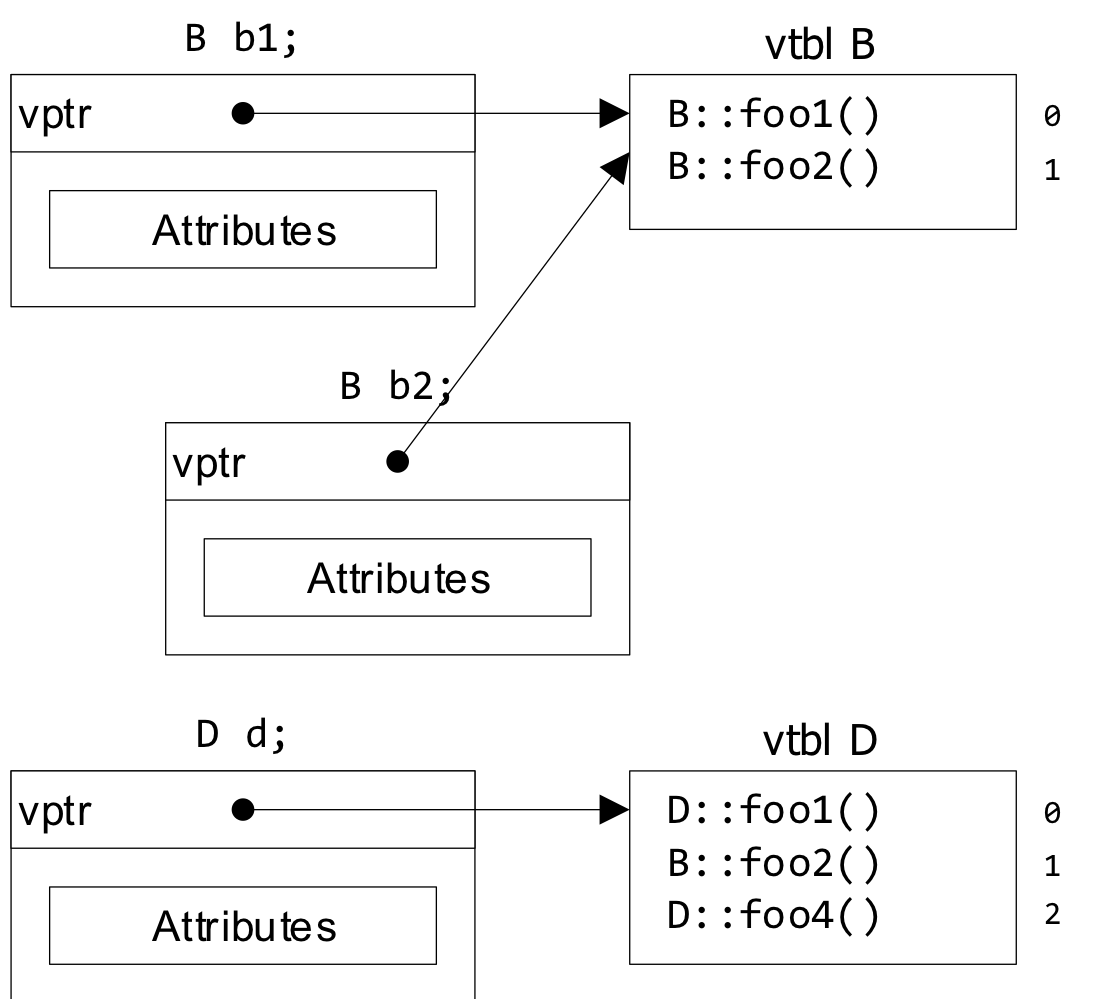
\includegraphics[width=\linewidth]{images/vtable.png}
\end{minipage}



\subsection{Abstrakte Klassen}

Wenn Klassen zwar festlegt, dass eine Methode da ist, diese aber noch nicht implementieren, nennt man das eine abstrakte Methode. 
Man spricht dann von einer abstrakten Klasse.
Eine abstrakte Methode wird in UML \textit{\textbf{kursiv}} dargestellt.
Es ist egal, ob die abstrakten Methoden selbst definiert sind oder geerbt. 
Abstrakte Klassen kann man nicht instanziieren.
Es gibt kein spezielles Schlüsselwort dafür, man weist der Methode bei Definition 0 zu: 

\lstinputlisting{code/03_Objektorientierung/abstraktemethode.cpp}

\subsection{Organisation der H files}

Generell gilt immer noch: Jedes H File hat ein Cpp File. 
Allerdings können Unterklassen in ein H File zusammengefasst werden, falls diese nicht allzu Umfänglich sind. 
Ansonsten sollte ein neues H File erstellt werden. 
Für abstrakte Klassen fällt die Implementierung in einem Cpp file weg.

\subsection{Mehrfachvererbung}

Folgender Vererbungszweig ist möglich:\\
\noindent
\begin{minipage}{0.38\columnwidth}
        \begin{tikzpicture}[
    node distance=0.4cm and 0.2cm,
]

    % Nodi
    \node[umlclass] (c1) {\textbf{C1}\nodepart{second}\nodepart{third}};
    
    \node[umlclass, below left=of c1] (c2) {\textbf{C2}\nodepart{second}print()\nodepart{third}};
    \node[umlclass, below right=of c1] (c3) {\textbf{C3}\nodepart{second}print()\nodepart{third}};
    
    % C4 posizionato centralmente sotto C2 e C3
    \node[umlclass, below=2cm of c1] (c4) {\textbf{C4}\nodepart{second}\nodepart{third}};

    % Connessioni
    \draw[inheritance] (c2) -- (c1);
    \draw[inheritance] (c3) -- (c1);
    \draw[inheritance] (c4) -- (c2);
    \draw[inheritance] (c4) -- (c3);

\end{tikzpicture} 
\end{minipage}
\begin{minipage}{0.62\columnwidth}
Solche Gebilde sind zwar möglich, sollten jedoch vermieden werden, da schnell sehr kompliziert und kaum lesbar. 
Es entsteht schnell Mehrdeutigkeit durch die verschiedenen Erbzweige.\\

Se nelle 2 classi parenti è definito un \cor{\textbf{metodo} con lo \textbf{stesso nome}}, è necessario
ridefinitrlo nella sottoclasse definendo il giusto comportamento (ad es. \lstinline[language=C++]|C1::print()|)
\end{minipage}

Bei der Definition einer Klasse können weitere Oberklassen mit einem Komma getrennt angegeben werden
\lstinputlisting{code/03_Objektorientierung/Mehrfachvererbung.cpp}\vspace{-1em}

\subsubsection{Diamond Problem}

\begin{itemize}
    \item \textbf{Il Problema}: Senza accorgimenti, \texttt{C4} conterrebbe due copie 
    separate di \texttt{C1} (tramite \texttt{C2} e tramite \texttt{C3}). 
    \cor{Generando ambiguità nell'accesso ai membri.}
    \item \textbf{La Soluzione (\textit{Virtual Inheritance})}:la parola 
    chiave \texttt{virtual} nelle classi intermedie (\texttt{C2} e \texttt{C3})
    istruisce il compilatore a creare un'unica istanza condivisa di \texttt{C1}.
    \item \textbf{Ordine di Inizializzazione}: Segue una priorità gerarchica:
    \begin{enumerate}
        \item \textbf{Base Virtuale}: \texttt{C1} viene inizializzata per prima.
        \item \textbf{Basi Non-Virtuali}: \texttt{C2} e poi \texttt{C3} (seguendo l'ordine di dichiarazione in \texttt{C4}).
        \item \textbf{Classe Derivata}: Il corpo del costruttore di \texttt{C4}.
    \end{enumerate}
\end{itemize}

\lstinputlisting[language=C++]{code/03_Objektorientierung/03_Objektorientierung_snippet_3.cpp}
\subsection{Static} 

Static im Zusammenhang mit Klassen bindet eine Methode oder ein Attribut an die Objektklasse und nicht an die Objektinstanz (ähnlich zu Python Klassenvariablen).


\subsubsection{Methoden}

Static Methoden müssen im Header-File deklariert und im Cpp-File definiert werden. 
Sie dürfen nur auf Static definierte Attribute zugreifen da \textbf{keine Objektinstanz vorhanden.} 
Hauptanwendungen sind Hilfsfunktionen wie Funktionsaufrufcounter oder Umrechnungsfunktionen. 
Bei der Deklaration wird der Klassennamen verwendet (siehe Bsp). 

\subsubsection{Attribute}

Static Attribute müssen im H deklariert \textbf{und im Cpp File} definiert werden. 
Sie werden verwendet für z.B. Objektspezifische Konstanten oder im Zusammenhang mit Static Counter. 
(\textit{class scope})

\subsubsection{Bsp}

\lstinputlisting{code/03_Objektorientierung/static.cpp}
        \section{Memorymanagement}

Es gibt verschiedene Gründe warum nicht immer gleich viel Speicher verwendet wird z.B. da nicht unbegrenzt vorhanden ist.
Speicher wird nur dann verwendet, wenn er wirklich gebraucht wird. 
Das Memorymanagement muss aktiv beachtet werden.
Es wird zwischen automatischen und manuellen Speichermanagement unterschieden. 

\subsection{Automatisch}

Automatisches Speichermanagement wird anhand der Lebenszeit einer Variable festgestellt und während dem Programmieren bereits festgelegt. 
Der Speicher liegt auf dem sogenannten \textbf{Stapel / Stack}.\\
Wird eine Funktion aufgerufen, werden die benötigten Variablen auf dem Stack definiert. 
Ebenso wird eine Returnadresse zur Funktion, die die Funktion aufgerufen hat abgelegt.
Wie die Daten angeordnet werden, ist Architektur-abhängig.
Wird die Funktion wieder verlassen, werden die Variablen vom Stack wieder entfernt und zur aufrufenden Funktion zurückgesprungen.  

\subsection{Manuell/dynamisch}

Man kann auch manuell Speicher anfordern. 
Zum Beispiel, falls zur Compilezeit nicht bekannt ist, wie viel Speicher gebraucht wird.
Dieser Speicher ist auf dem sogenannten \textbf{Haufen / Heap}.\\
Der Heap ist ein Speicherbereich, der vom Betriebssystem bereitgestellt und verwaltet wird.\\
Zur Laufzeit wird Speicher dynamisch angefordert. 
Dieser bleibt so lange belegt bis dieser Manuell wieder freigegeben wird.\\
Es kann aber auch sein, falls der Speicher stark fragmentiert ist, das kein Speicher bereitgestellt werden kann. 
Generell ist bei sehr vollem Speicher das Arbeiten erschwert.

\subsubsection{Memory leaks}

Falls ein Programm unkontrolliert Speicher aufnimmt oder den ihm zur Verfügung gestellte nicht wieder freigibt, spricht man von einem Speicherleck. 
Diese sind zu verhindern da diese zu einer Systemüberlastung und Abstürzen führen.

\example{}
\begin{minipage}{0.5\columnwidth}
  \lstinputlisting[language=C++]{code/04_Memorymanagement/memory_leaks.cpp}
\end{minipage}
\begin{minipage}{0.5\columnwidth}
  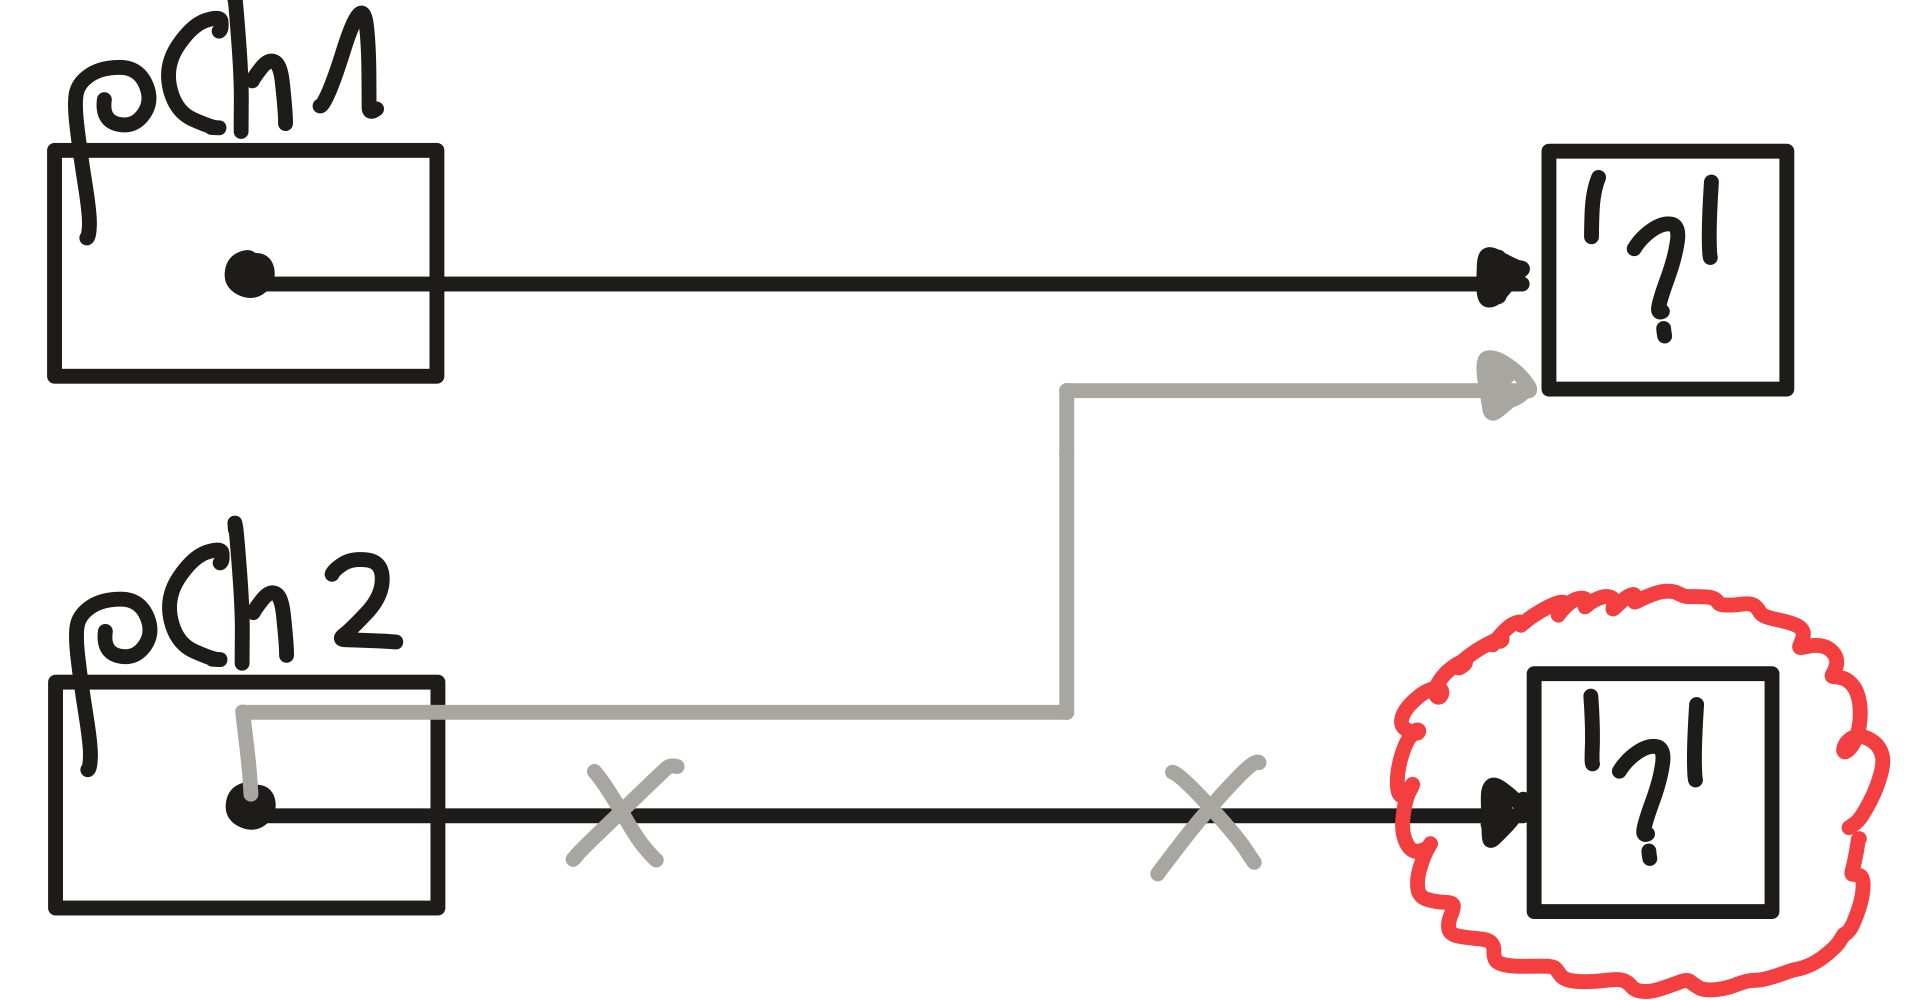
\includegraphics[width=\linewidth]{images/memory_leak.png}
\end{minipage}

\subsection{Speichermanagement funktionen}

Es gibt einige Funktionen für Speichermanagement. In C und C++ sind diese leicht verschieden. 
Generell geben diese einen Pointer zurück, welcher auf freien Speicher zeigt. 
\textbf{Diese müssen immer auf einen Nullpointer geprüft werden, da keine Garantie vorhanden ist, ob überhaupt Speicher vorhanden ist!}
Generell sollte mit solchen Pointer immer misstrauisch gearbeitet werden und nach Abschluss immer wieder freigegeben werden.

\subsubsection{C: \texttt{malloc()},  \texttt{calloc()}, \texttt{free()}}

\textbf{malloc()} gibt einen Voidpointer(pointercasting nicht vergessen) zurück welche auf eine angeforderte Grösse an Bytes Speicher zeigt. 
Der Speicher ist \textbf{nicht} initialisiert
\textbf{calloc()} macht dasselbe, initialisiert aber den Speicher auf 0.\\
\textbf{free()} gibt den Speicherbereich wieder frei.

\lstinputlisting{code/04_Memorymanagement/mem_mngmt_c.c}

Falls kein Speicher allokiert werden kann, wird ein NULL-pointer zurückgegeben.

\subsubsection{C++: \texttt{new}, \texttt{delete}, \texttt{new[]}, \texttt{delete[]} (Operatoren)}

Der \textbf{new}-Operator erstellt ein Pointer welcher auf die mitgegebene Grösse zeigt.

\textbf{new[ ]} macht dasselbe, ausser das dieser ein Array zurückgibt.

\textbf{delete} / \textbf{delete[ ]} gibt den Speicher wieder frei. 
Dieser kann auch auf den Nullpointer ausgeführt werden. 
Dieser ist \texttt{Delete} egal.

\lstinputlisting{code/04_Memorymanagement/mem_mngmt_cpp.cpp}

\subsection{Speicheraufbau}

Der Speicheraufbau bildlich dargestellt sieht ungefähr so aus:

\begin{center}
    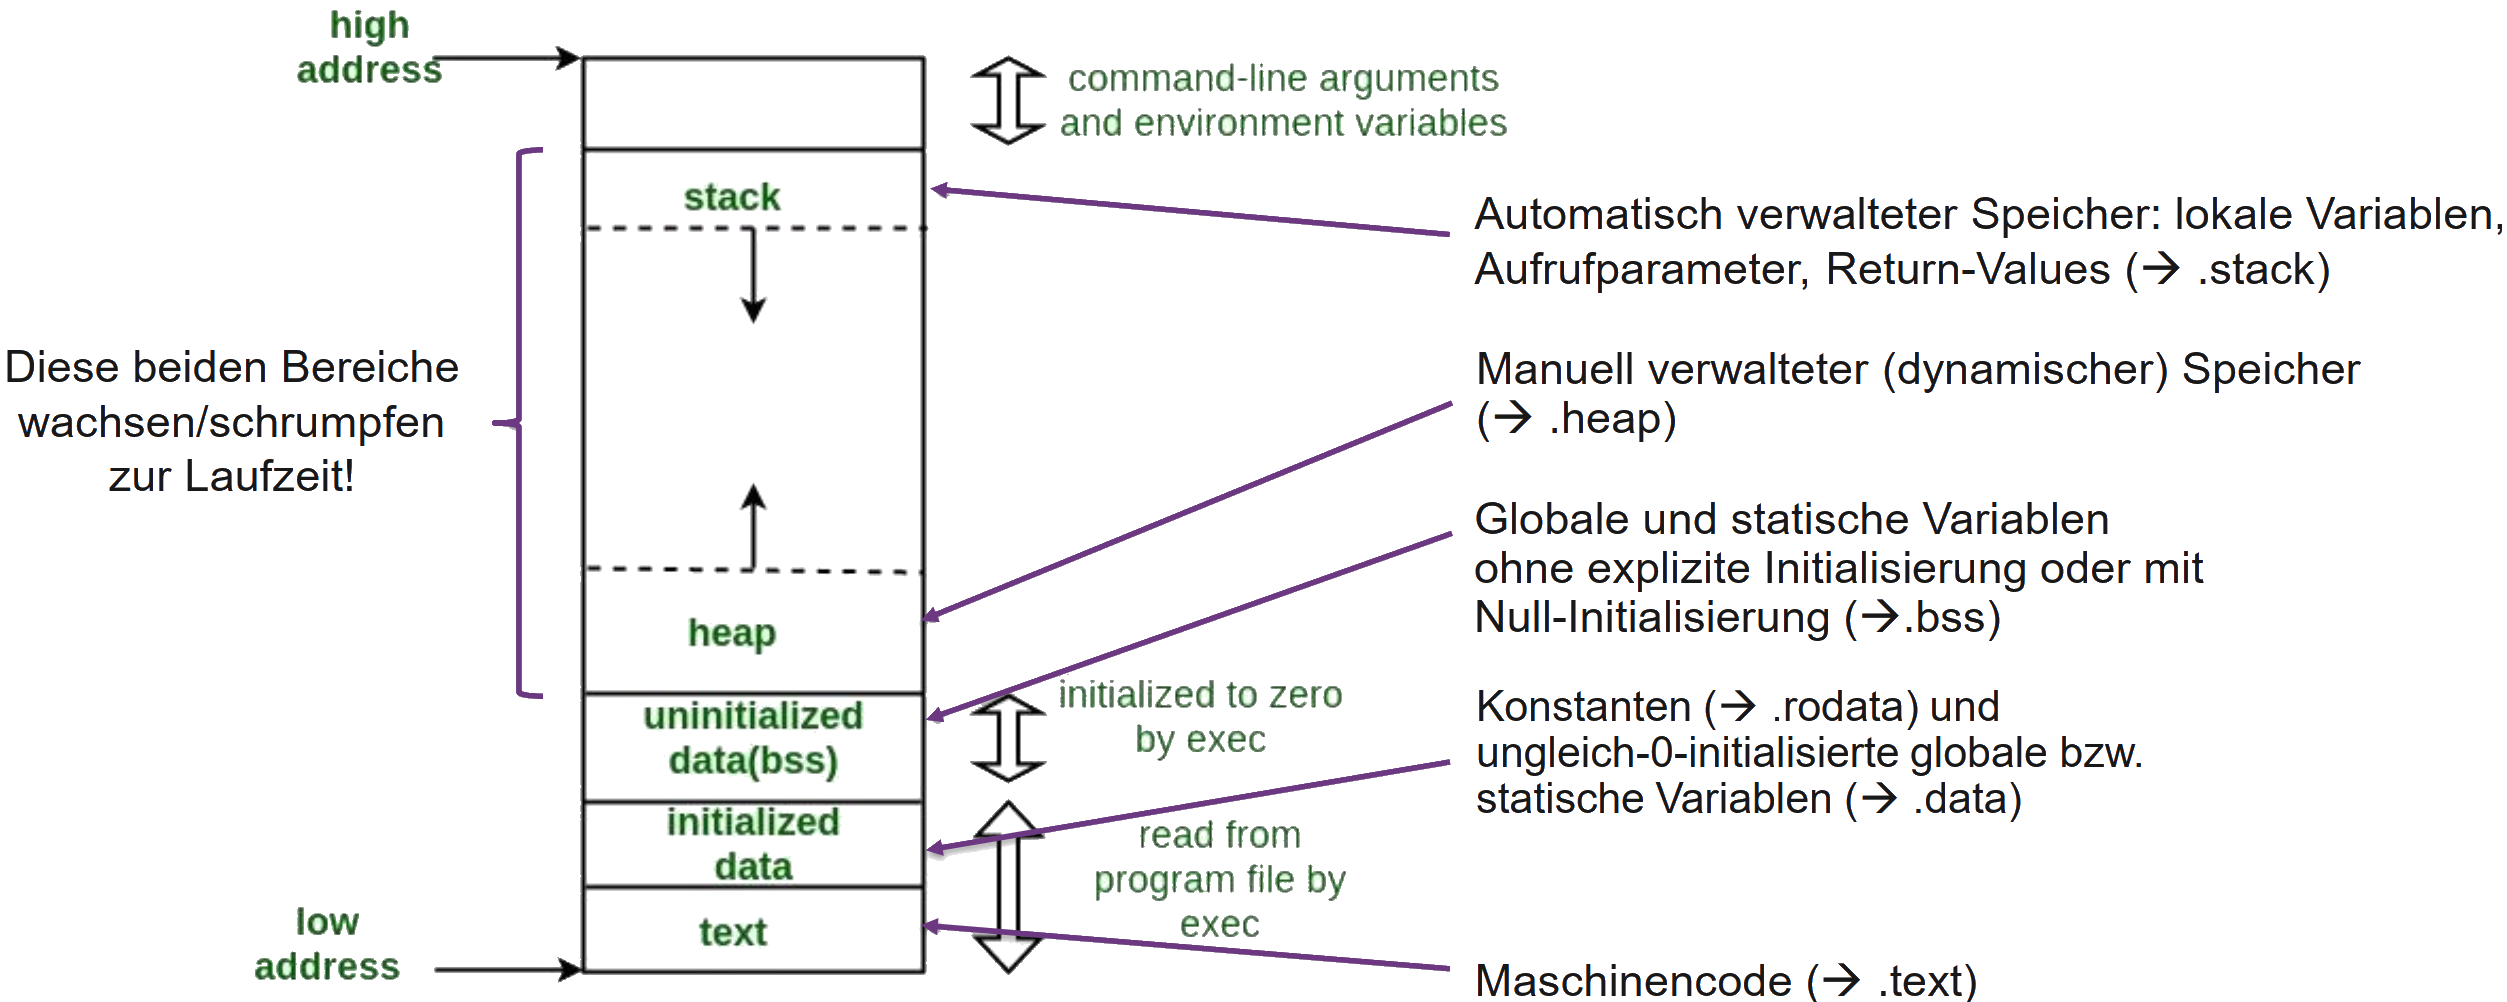
\includegraphics[width=\columnwidth]{images/memorylayout.png}  
\end{center}

Je nach Architektur kann es auch sein, dass die hohen und tiefen Adressen anders herum sind.

\subsection{Referenzen}
Una referenza è un \textbf{alias} (un nome alternativo) per una variabile o una cella di memoria già esistente. Rappresentano una versione più moderna, sicura e ristretta dei puntatori.

\subsubsection{Caratteristiche Principali}
\begin{itemize}
    \item \textbf{Inizializzazione obbligatoria:} Deve essere inizializzata subito: \texttt{int\& r = x;}
    \item \textbf{Immutabilità:} Non può essere modificata per puntare a un altro oggetto dopo la definizione.
    \item \textbf{Sicurezza:} Non possono essere mai non inizializzate e non hanno mai il valore \texttt{nullptr}.
    \item \textbf{Efficienza:} Possono risiedere nei registri della CPU e non occupano sempre memoria fisica. L'operatore \texttt{sizeof()} restituisce la dimensione del tipo a cui la referenza punta.
    \item \textbf{Sintassi:} Vengono utilizzate come variabili normali, senza necessità di dereferenziazione.
    \item \textbf{Limitazione con gli Array:} Le referenze non possono essere usate per scorrere gli array tramite aritmetica (incremento/decremento). Per questo scopo, i \textbf{puntatori} rimangono indispensabili.
\end{itemize}

\subsubsection{Confronto: Value vs Reference}
\begin{center}
\begin{tabular}{@{}lll@{}}
\toprule
\textbf{Caratteristica} & \textbf{Call by Value} & \textbf{Call by Reference} \\ \midrule
Copia dei dati          & Sì (costoso per oggetti grandi) & No (passa l'alias) \\
Modifica originale      & No                             & Sì \\
Sintassi                & \texttt{void f(int a)}         & \texttt{void f(int\& a)} \\ \bottomrule
\end{tabular}
\end{center}

\subsubsection{Best Practices}
L'utilizzo delle referenze riduce drasticamente i rischi di errori rispetto ai puntatori. Tuttavia, i puntatori rimangono necessari in casi specifici:
\begin{itemize}
    \item \textbf{Gestione degli Array:} Un array "decade" naturalmente in un puntatore al suo primo elemento (\textit{pointer decay}), rendendo i puntatori lo strumento standard per iterare o manipolare blocchi di memoria contigui.
    \item \textbf{Programmazione Low-level:} Necessaria per l'interazione diretta con l'hardware o allocazione dinamica manuale (\texttt{new}/\texttt{delete}).
\end{itemize}

\lstinputlisting{code/04_Memorymanagement/referenz.cpp}

\subsection{Speicherplatzbedarf von Objekten}

Eine Unterklasse braucht immer mindestens so viel speicher wie eine Oberklasse.

\subsubsection{Zuweisungen}

Zuweisungen von Oberklasse zu Unterklasse sind in der regel möglich da alle geerbten Attribute ja vorhanden sind. 
Umgekehrt geht das allerdings nicht, da der Speicher dafür nicht initialisiert ist.

\subsubsection{Slicing Problem}

\begin{itemize}
    \item \textbf{Definizione:} Si verifica quando un oggetto di una sottoclasse viene passato \textbf{per valore} a una funzione che si aspetta la superclasse.
    \begin{itemize}
        \item Viene invocato il \textit{Copy-Constructor} della superclasse.
        \item Solo la parte "base" dell'oggetto viene copiata; le estensioni della sottoclasse vengono perse (slicing).
    \end{itemize}
    \item \textbf{Conseguenza:} All'interno della funzione, l'oggetto si comporta esclusivamente come un'istanza della classe base, perdendo ogni comportamento polimorfico.
    \item \textbf{Soluzione:} Utilizzare sempre il passaggio \textbf{per referenza} (\texttt{const T\&}) o tramite puntatori. Questo preserva l'integrità dell'oggetto originale e permette il corretto funzionamento dei metodi \texttt{virtual}.
\end{itemize}

\subsection{Type Casting}\vspace{-1em}

\begin{center}
    \rotatebox{90}{%            
    \resizebox{1.5 \columnwidth}{!}{%
    \begin{tabular}{|c|l|l|l|}
        \hline
        {\color{blue} Cast:} &
          \multicolumn{1}{c|}{{\color{blue} Anwendungsbereiche}} &
          \multicolumn{1}{c|}{{\color{blue} Wissenswertes}} &
          \multicolumn{1}{c|}{{\color{blue} Beispiele}} \\ \hline
        {\color{blue} \begin{tabular}[c]{@{}c@{}}implizit: \\ kein Cast\end{tabular}} &
          \begin{tabular}[c]{@{}l@{}}• Numerische Typen u. bool\\ (ggf. mit Warnung, falls Wertebereich\\ möglicherweise nicht ausreicht)\\ • Objektinstanzen einer Unterklasse in\\ einer Variablen vom Typ der\\ Oberklasse speichern (Upcast).\\ • Pointertypen, deren Umkonvertierung\\ «ungefährlich» ist – die genauen\\ Regeln sind ziemlich kompliziert.\end{tabular} &
           &
          \begin{tabular}[c]{@{}l@{}}1. {\color{codeGreen}signed char} a = 1;\\ {\color{codeGreen}int} b = a;\\ \\ 2. {\color{codeGreen}int} a = 1;\\ {\color{codeGreen}char} b = a; {\color{blue}// ggf. mit Warnung}\\ \\ 3. Bird b;\\ Animal a = b; {\color{blue}// Upcast: a ist ein Animal}\end{tabular} \\ \hline
        {\color{blue} static} &
          \begin{tabular}[c]{@{}l@{}}• Alles, was implizit möglich ist,\\ unterdrückt dabei etwaige Warnungen.\\ • Pointer- und Referenz-Typen auf\\ Instanzen von Ober- und\\ Unterklassen in beide Richtungen\\ umwandeln: Upcast und\\ Downcast (\textbf{ohne Typprüfung} zur\\ Laufzeit, Auswertung\\ ausschliesslich zur \textbf{Compilezeit})\end{tabular} &
          \begin{tabular}[c]{@{}l@{}}Per convertire un tipo intero più \\ grande in uno più piccolo, il \\ compilatore semplicemente "taglia" \\ i bit in eccesso, mantenendo solo \\ quelli meno significativi (LSB).\end{tabular} &
          \begin{tabular}[c]{@{}l@{}}1. {\color{codeGreen}int} a = 1;\\ {\color{codeGreen}char} b = {\color{codeGreen}static\_cast}\textless{}{\color{codeGreen}char}\textgreater{}(a);\\ 2. Bird* b = {\color{codeGreen}new} Bird;\\ Animal* a = b; {\color{blue}// geht implizit!}\\ Bird* c = {\color{codeGreen}static\_cast}\textless{}Bird*\textgreater{}(a);\\ {\color{blue}/* Braucht einen down-Cast} , \\ {\color{codeGreen}weil nicht jedes Animal ein Bird ist!*/}\end{tabular} \\ \hline
        {\color{blue} dynamic} &
          \begin{tabular}[c]{@{}l@{}}• Pointer- und ReferenzTypen auf \\ Instanzen von\\ \textbf{polymorphen} Ober- und\\ Unterklassen in beide\\ Richtungen umwandeln:\\ Upcast und Downcast (\textbf{mit}\\ Typprüfung per RTTI zur\\ Laufzeit)\end{tabular} &
          \begin{tabular}[c]{@{}l@{}}Unterstützt ausserdem einen\\ Upcast für Pointer- und\\ Referenztypen auf nichtpolymorphe Klassen\\ (normalerweise machen wir dies aber \\ implizit oder verwenden einen static\_cast!)\\ Falls der dynamic\_cast \textbf{fehlschlägt}, liefert \\ er bei Pointer-Typen den Wert\\ \textbf{nullptr}, bei Referenzen wird\\ eine \textbf{std::bad\_cast-Exception} geworfen\end{tabular} &
          \begin{tabular}[c]{@{}l@{}}Animal* a = {\color{codeGreen}new} Ant;\\ Bird* b = {\color{codeGreen}dynamic\_cast}\textless{}Bird*\textgreater{}(a);\\ {\color{blue}/* Der Dynamic Cast wird}\\ {\color{blue}immer zur Laufzeit ausgewertet.  dh:}\\ {\color{blue}b ==nullptr */}\end{tabular} \\ \hline
        {\color{blue} const} &
          \begin{tabular}[c]{@{}l@{}}verändert die \texttt{constness} und/oder\\ \texttt{volatile-ness} des\\ Ziels eines Pointer oder Referenz Typs.\end{tabular} &
           &
          \begin{tabular}[c]{@{}l@{}}{\color{codeGreen}const int} val = 10; \\ {\color{codeGreen}const int} *ptr = \&val; \\ {\color{codeGreen}int} *ptr1 = {\color{codeGreen}const\_cast} \textless{}{\color{codeGreen}int} *\textgreater{}(ptr);\end{tabular} \\ \hline
        {\color{blue} reinterpret} &
          \begin{tabular}[c]{@{}l@{}}• Konvertiert zwischen beliebigen Pointer-Typen \\ sowie zwischen beliebigen Pointer und int-Typen \\\textbf{ohne Typprüfung}.\\ • Kann auch mit Referenz-Typen\\ umgehen.\end{tabular} &
          \begin{tabular}[c]{@{}l@{}}Achtung: erzeugt\\ plattformspezifisches Verhalten\end{tabular} &
          \begin{tabular}[c]{@{}l@{}}Animal* a = {\color{codeGreen}new} Ant;\\ \\ {\color{codeGreen}uint8\_t}* b =\\ {\color{codeGreen}reinterpret\_cast}\textless{}{\color{codeGreen}uint8\_t}*\textgreater{}(a);\end{tabular} \\ \hline
        \end{tabular}%
    }
    }          
\end{center}

Die C Syntax für Casting sollte nicht mehr verwendet werden da meistens nicht optimales verhalten. 

\subsection{Templates}

\begin{itemize}
\item \textbf{Indipendenza dal tipo:} Consentono di scrivere codice generico utilizzando dei \textbf{placeholder} (segnaposti) al posto di tipi specifici.
\item \textbf{Sicurezza dei tipi (Type Safety):} A differenza del C 
(\lstinline|void*|), i template garantiscono un controllo dei tipi tramite \textit{early binding} in fase di compilazione.
\item \textbf{Parametri di istanziazione:} Oltre ai tipi, è possibile 
passare anche delle \textbf{costanti} come parametri del template 
\item \textbf{Versatilità:} Possono essere applicati sia a \textbf{classi} che a 
\textbf{funzioni}.
\item \textbf{Valutazione a tempo di compilazione:} Il compilatore genera il codice 
effettivo durante la fase di \textbf{compile-time}.
\item \textbf{Struttura e File:} Richiedono dichiarazione, definizione e parametri; 
solitamente vengono \crd{definiti interamente negli \textbf{header file} (.h / .hpp).}
\item \textbf{Generazione del codice:} Il compilatore crea una copia separata della 
funzione o classe per ogni \textbf{diverso tipo} utilizzato.
\item \textbf{Zero Dead Code:} Se un template non viene mai utilizzato nel codice, 
non viene generata alcuna istruzione nel binario finale
\item \textbf{Footprint di memoria e Code Bloat:} L'istanziazione per molteplici tipi, 
oppure l'uso eccessivo della keyword \lstinline|inline| per definizioni lunghe, 
può causare \textit{code bloat}.
\end{itemize}

\subsubsection{Implementation}

Die Typendefinitionen sind dann durch das T zu ersetzen. 

\lstinputlisting{code/04_Memorymanagement/templatesswap.cpp}\vspace{-1.5em}

\begin{center}
  \cor{As the dimension of the paramters is unknow ALWAYS use references}
\end{center}

\subsubsection{Syntax}

\lstinputlisting{code/04_Memorymanagement/templatesyntax.cpp}\vspace{-0.5em}

\subsubsection{Instanziierung}

L'istanziazione è il processo con cui il compilatore genera codice macchina concreto\smallbreak

\begin{itemize}
    \item \textbf{Implicita:} compilatore deduce il tipo dai parametri passati 
    \textbf{Nota bene:} il tipo di ritorno non viene mai considerato per la deduzione
    \item \textbf{Esplicita:} Il tipo viene specificato manualmente tra parentesi angolari 
\end{itemize}\smallbreak

\textbf{Klassentemplates} (\verb|<>| obbligatori):\\
tipo sempre specificato per permettere al compilatore di determinare l'ingombro in memoria.\\
\lstinline[language=C++]|Stack<int, 10> s1; // Istanzia uno Stack di 10 interi|

\textbf{Funktionstemplates} (\verb|<>| opzionali se deducibili):\\
Se il tipo è chiaro dai parametri, le parentesi angolari possono essere omesse.\\
\lstinline[language=C++]|int i = minimum(iF, size); // Deduzione implicita del tipo int|
\lstinline[language=C++]|int i = minimum<int>(iF, size); // Qualificazione esplicita|

\subsubsection{Overloading}

I template di funzione possono essere sovraccaricati (overloaded) con altri template o con funzioni "normali". In caso di chiamate omonime, il compilatore valuta le funzioni compatibili, istanzia quelle dei template, le aggiunge alle funzioni normali disponibili e infine seleziona la variante che offre il \textit{match} migliore con i tipi dei parametri passati.

\subsubsection{Kompilierung und Code-Organisation}
\begin{itemize}
    \item \textbf{Header-Only:}  il compilatore deve 'vedere' la definizione per ogni 
    traduzione. Lo svantaggio principale è l'\textbf{aumento dei tempi di compilazione} 
    \item \textbf{Explicit Instantiation (.cpp):} Per ridurre i tempi di compilazione, 
    è possibile spostare la definizione in un file \verb|.cpp| e forzare l'istanziazione 
    per tipi specifici (es. \lstinline|template class Stack<int>;|). 
\end{itemize}

\section{Exceptions (Ausnahmen)}
\begin{itemize}
    \item \textbf{Error (Fehler):} Errore di implementazione. Dovrebbe essere rimosso durante il testing/verifica.
    \item \textbf{Exception (Ausnahme):} Condizione anormale che può verificarsi a runtime (es. file non trovato, timeout di rete).
\end{itemize}


\subsection{Meccanismo: Throw e Catch}
Un'eccezione è un oggetto lanciato con la keyword \texttt{throw} e intercettato da un blocco \texttt{catch}.

\begin{itemize}
    \item \textbf{Throw by value:} Le eccezioni dovrebbero sempre essere lanciate per valore.
    \item \textbf{Catch by const reference:} Per evitare copie inutili e il problema dello \textit{slicing} degli oggetti, intercettare sempre per riferimento costante.
    \item \textbf{Stack Unwinding:} lanciata un'eccezione, il programma distrugge 
    automaticamente tutti gli oggetti (chiama i distruttori) e salta 
    \textbf{al primo handler compatibile}.
\end{itemize}

\lstinputlisting[language=C++]{code/04_Memorymanagement/exceptionGenerellSyntax.cpp}\vspace{-1em}

\subsection{Propagazione (Exception Propagation)}
Se un'eccezione non viene gestita localmente, può essere passata "verso l'alto" (es. fino al livello applicativo) dove può essere presa una decisione sensata (Grundsatz: gestire solo ciò che si può decidere).
\begin{itemize}
    \item All'interno di un blocco \texttt{catch}, l'istruzione \texttt{throw;} (senza argomenti) ri-lancia l'eccezione corrente alla funzione chiamante.
\end{itemize}

\subsection{Gerarchia e Ordine dei Catch}
In C++, le eccezioni sono organizzate gerarchicamente sotto la classe base \texttt{std::exception} (definita in \texttt{<exception>}).

\begin{itemize}
    \item \textbf{logic\_error: \crd{DA NON USARE}} Errori prevenibili in fase di sviluppo
    \item \textbf{runtime\_error:} Errori non prevedibili dovuti a eventi esterni\\
    (es. \texttt{overflow\_error}, \texttt{system\_error}, \crd{includere \texttt{stdexcept}}).
\end{itemize}

\medbreak

\textbf{\color{orange}Regola cruciale:} Gli handler devono essere ordinati dal più specifico al più 
generico nel codice. \texttt{std::exception} o il catch-all \texttt{...} deve essere l'ultimo.

\begin{lstlisting}{language=C++}
catch(...) {
  // Catch everything
}
\end{lstlisting}

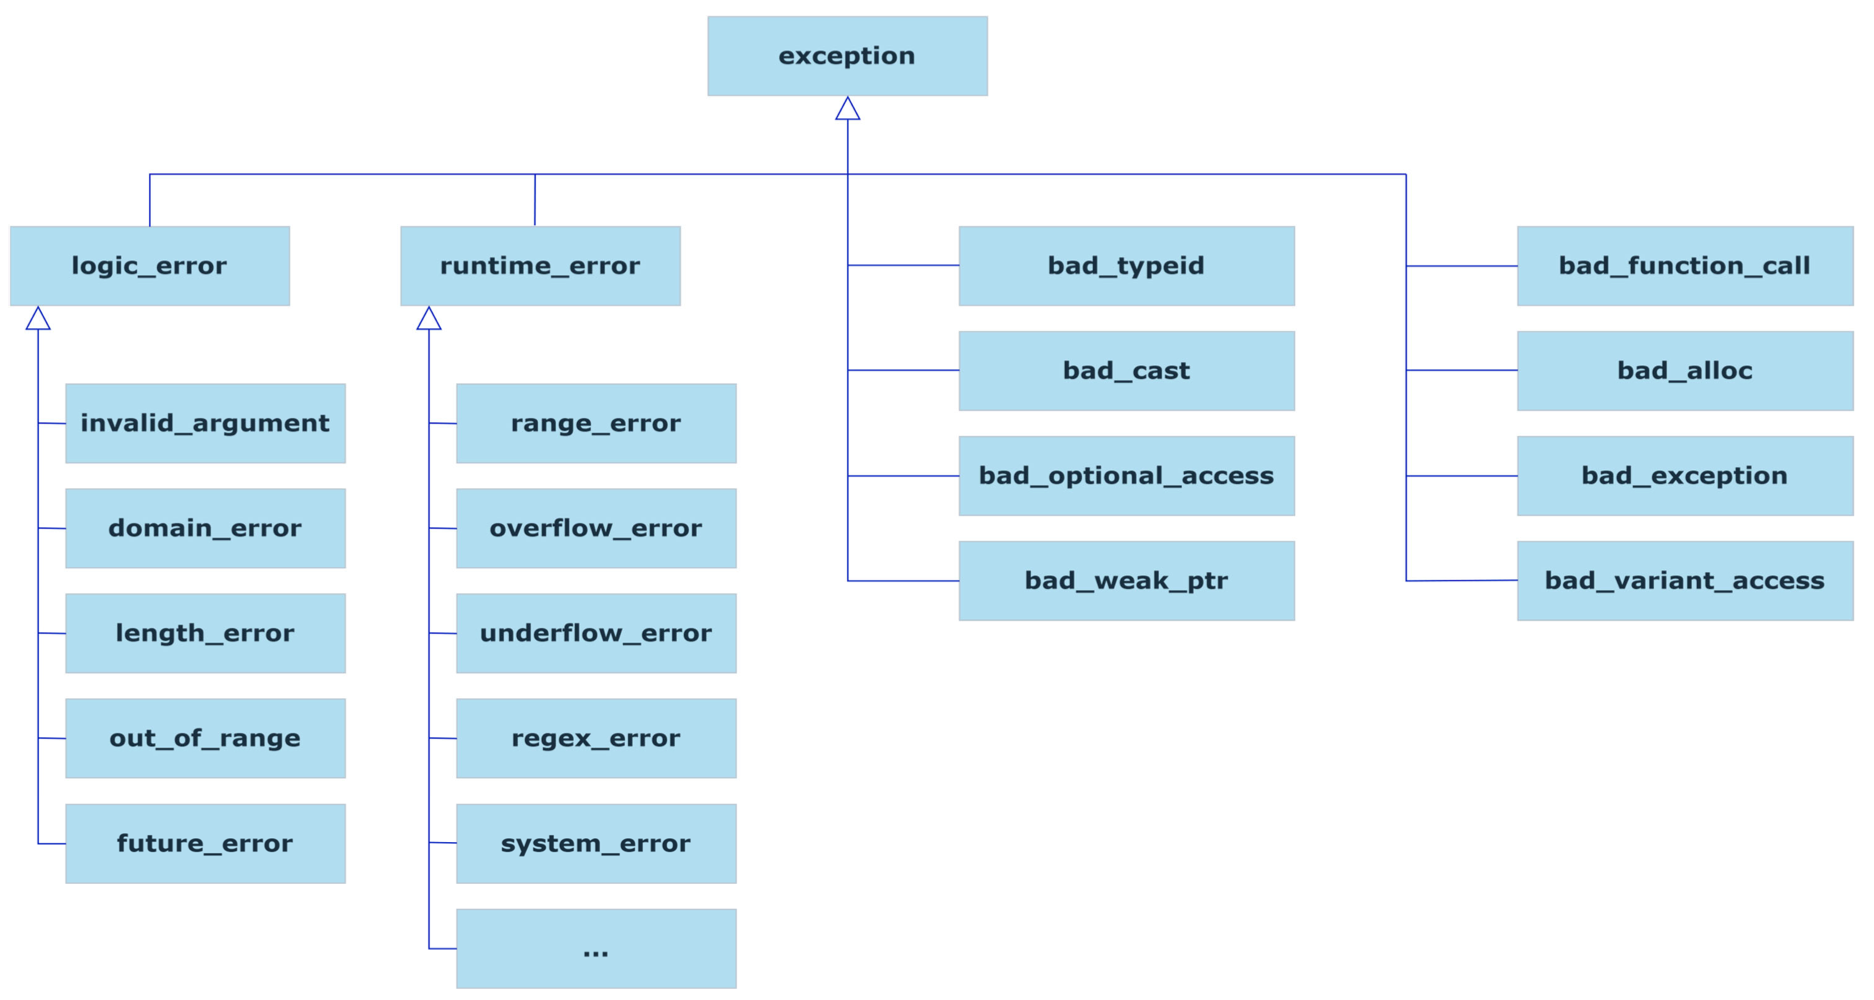
\includegraphics[width=\linewidth]{images/exception_hierarchie.png}

\example{}
\lstinputlisting[language=C++]{code/04_Memorymanagement/catchcatcher.cpp}\vspace{-1em}

\subsection{Eccezioni non gestite}
Se non viene trovato alcun handler nel \textit{Call Stack}:


\begin{enumerate}
    \item Viene chiamata la funzione \texttt{std::terminate}.
    \item \texttt{std::terminate} richiama un \texttt{terminate\_ handler} (di default \texttt{std::abort}).
    \item Il programma termina bruscamente (no esecuzione dei distruttori)
\end{enumerate}\smallbreak

È possibile personalizzare questo comportamento tramite \texttt{std::set\_terminate()}.

\subsection{noexcept}
\begin{itemize}
    \item \textbf{noexcept:} Introdotto con C++11, indica che una funzione garantisce di non lanciare eccezioni. È utile per l'ottimizzazione del compilatore.
    \item \textbf{Operatore noexcept(expr):} Restituisce \texttt{true} se l'espressione è specificata come \texttt{noexcept}.
\end{itemize}

\lstinputlisting[language=C++]{code/04_Memorymanagement/noexcept.cpp}\vspace{-1em}

\subsection{C++ e Low-Level Exceptions}
A differenza di Java o C\#, il linguaggio C++ \textbf{non} effettua il \textit{mapping}
automatico delle eccezioni di basso livello (come la divisione per zero) in eccezioni 
del linguaggio.
\smallskip

Handling con \texttt{catch(...) \{ \}} 

\section{STD Library}
\subsection{array}
\begin{itemize}
\item \textbf{Definizione:} \texttt{std::array<T, size>} è un contenitore a dimensione fissa implementato come classe template.
\item \textbf{Dimensione:} A differenza dei classici array in stile C, \texttt{std::array} conosce la propria dimensione tramite la funzione membro \texttt{.size()}.
\item \textbf{Accesso ai dati:} È possibile accedere agli elementi utilizzando la classica notazione a parentesi quadre \texttt{[]}.
\item \textbf{Sicurezza:} Il metodo \texttt{.at()} fornisce un accesso sicuro con controllo dei limiti, lanciando un'eccezione \lstinline|std::out_of_range| in caso di accesso non valido.
\item \textbf{Integrazione:} Funziona in modo ottimale con le moderne funzionalità del C++, inclusi i cicli \textit{range-based for}.
\end{itemize}

\subsection{vector}
std:vector ist ein Klassentemplate welches die Kapazität selbständig bei Bedarf erweitert.
\lstinputlisting{code/04_Memorymanagement/vector.cpp}
        \section{Makefile}

In eine Makefile können Abhängingkeiten definiert werden\\
Wenn eine Datei geändert wurde, dann werden alle Operationen ausgeführt mit den Dateien, welche von
dieser geänderten Datei abhängen

\textbf{Il makefile viene eseguito dal basso verso l'alto!}

\subsection{Variabili}
Le variabili vengono definite come \texttt{NAME = valore} e richiamate con \texttt{\$(NAME)}. 
Esempio:
\begin{lstlisting}[language=make]
CC = clang
CFLAGS = -c -Wall
\end{lstlisting}

\subsection{Regole e Dipendenze}
La sintassi fondamentale è:
\begin{center}
\texttt{Target: Dipendenze} \\
\texttt{\quad [TAB] Comando Shell}
\end{center}

\begin{itemize}
    \item Il comando viene eseguito solo se una dipendenza è più recente del target.
    \item Il simbolo '\texttt{\$@}' rappresenta il nome del target corrente.
    \item È obbligatorio l'uso del tasto TAB per i comandi.
\end{itemize}

\subsection{Esempio Pratico}
\begin{center}
    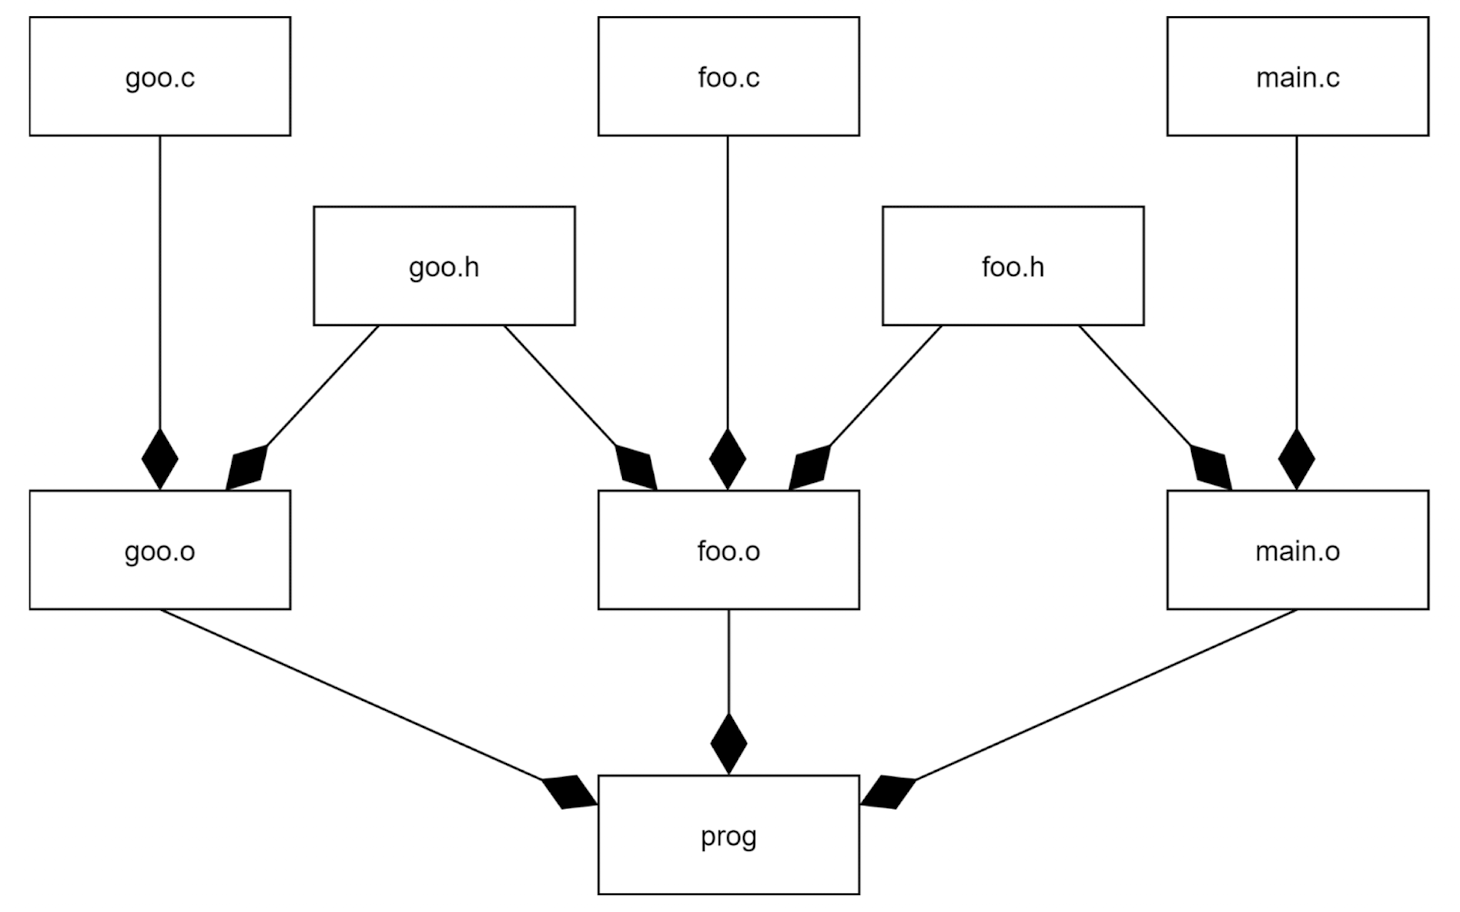
\includegraphics[width=0.78\columnwidth]{images/dateien_abhaengigkeiten.png}
\end{center}\vspace{-1.5em}

\lstinputlisting[language=makefile]{code/05_makefiles/makefile}
        \newpage
        \section{Anhang}

\subsection{Styleguide}

\begin{itemize}[itemsep=1pt, parsep=0pt]
    \item \textbf{Variablen, Konstanten}
    \begin{itemize}[itemsep=1pt, parsep=0pt]
        \item mit Kleinbuchstaben beginnen
        \item erster Buchstaben von zusammengesetzten Wörtern ist gross (mixed case)
        \item keine Underscores
    \end{itemize}
    Beispiele : counter, maxSpeed
    \item \textbf{Funktionen}
    \begin{itemize}[itemsep=1pt, parsep=0pt]
        \item mit Kleinbuchstaben beginnen
        \item erster Buchstaben von zusammengesetzten Wörtern ist gross (mixed case)
        \item Namen beschreiben Tätigkeiten
        \item keine Underscores
    \end{itemize}
    Beispiele : getCount(), init(), setMaxSpeed()
    \item \textbf{Klassen, Strukturen, Enums}
    \begin{itemize}[itemsep=1pt, parsep=0pt]
        \item mit Grossbuchstaben beginnen
        \item erster Buchstaben von zusammengesetzten Wörtern ist gross (mixed case)
        \item keine Underscores
        \item Namen beschreiben Dinge
    \end{itemize}
    Beispiele : MotorController, Queue, Color
\end{itemize}

\subsection{Code beispiele}
\subsubsection{String formatting}
Utilizza gli stream di output per costruire stringhe in memoria. È sicuro perché gestisce la memoria dinamicamente.

\lstinputlisting[language=C++]{code/99_anhang/99_anhang_snippet_1.cpp}

Rappresenta lo standard moderno. Combina la sintassi concisa di \texttt{printf} con la sicurezza degli stream.

\lstinputlisting[language=C++]{code/99_anhang/99_anhang_snippet_2.cpp}

\subsubsection{Ctor un dtor}
\lstinputlisting[language=c++]{code/99_anhang/ctor_dtor_anhang.cpp}

\subsection{Ritorno per Riferimento e Method Chaining}
\begin{itemize}
    \item \textbf{Meccanismo:} Una funzione restituisce un riferimento all'oggetto stesso
    utilizzando \texttt{return *this;}. Il tipo di ritorno deve 
    essere una referenza (es. \texttt{Complex\&}).
    \item \textbf{Kaskadierung (Cascading):} Permette di chiamare più metodi in 
    sequenza sulla stessa istanza in un'unica riga: \texttt{obj.funz1().funz2();}.
    
    \crd{Tramite ritorno \textit{by-value} funz2 verrebbe eseguita su un oggetto \textit{tmp}}
    \item \textbf{Efficienza:} A differenza del ritorno per valore, 
    non viene creata alcuna copia dei dati (nessun oggetto temporaneo \textit{tmp}), 
    risparmiando risorse 
    \item \textbf{Persistenza:} Le modifiche effettuate nella catena agiscono 
    direttamente sull'oggetto originale e non su una sua copia destinata alla distruzione.
\end{itemize}

\lstinputlisting[language=c++]{code/99_anhang/method_chaining.cpp}

\subsubsection{Vergleich von Gleitkommazahlen (double)}
Beim Vergleich von \texttt{double}-Werten sollte aufgrund von Rundungsfehlern \textbf{niemals 
der Operator \texttt{==} direkt verwendet werden}. 

Stattdessen wird geprüft, ob die absolute Differenz zwischen zwei Werten kleiner als eine definierte Toleranz 
(Epsilon) ist.

\lstinputlisting[language=C++]{code/99_anhang/99_anhang_snippet_3.cpp}

\subsection{Parametri Template Non-Tipo (Static Allocation)}

I template accettano valori costanti (es. \texttt{std::size\_t N}) valutati a 
\textbf{compile-time}. Questo è l'unico modo per definire la dimensione di array statici 
(\texttt{T data[N]}) mantenendo la flessibilità del codice.

In C++, il compilatore deve conoscere l'ingombro esatto di un oggetto nello \textbf{Stack}
per generare istruzioni macchina con \textit{offset} fissi. Se \texttt{N} fosse una
variabile, il compilatore non saprebbe quanto spazio riservare automaticamente e 
l'allocazione fallirebbe.

\subsubsection{Allocazione Statica vs Dinamica}
Senza la risoluzione a tempo di compilazione, il compilatore non potrebbe riservare lo spazio nello \textbf{Stack}, obbligando all'uso della memoria \textbf{Heap} (più lenta).

\resizebox{\columnwidth}{!}{
\begin{tabular}{|l|l|l|}
\hline
\textbf{Caratteristica} & \textbf{Via Template (Statico)} & \textbf{Via Costruttore (Dinamico)} \\ \hline
\textbf{Vincolo Size}   & Costante a compile-time & Variabile a run-time \\ \hline
\textbf{Memoria}        & Stack (Veloce, fissa)   & Heap (Flessibile, lenta) \\ \hline
\textbf{Gestione}       & Automatica (No memory leaks) & Manuale (\texttt{new}/\texttt{delete}) \\ \hline
\textbf{Effetto Tipo}   & \texttt{Class<10>} $\neq$ \texttt{Class<20>} & Il tipo rimane identico \\ \hline
\end{tabular}}\vspace{1em}

\lstinputlisting[language=C++]{code/99_anhang/99_anhang_snippet_4.cpp}

\subsection{Inline Functions e Templates}

\begin{itemize}
    \item \textbf{Inlining Implicito:} Tutte le funzioni (template e non) definite direttamente all'interno della dichiarazione di una classe (\textit{in-class}) sono considerate \texttt{inline} automaticamente dal compilatore.
    \item \textbf{Inlining Esplicito:} Le funzioni template definite al di fuori della classe (\textit{out-of-class}), anche se collocate nello stesso file header, \textbf{non} sono \texttt{inline} di default. Per renderle tali, la keyword \texttt{inline} deve essere inserita tra il tag \texttt{template} e il tipo di ritorno.
    \item \textbf{Vantaggi e Limiti:} L'inlining elimina l'overhead della chiamata a funzione (\textit{zero overhead}), ma è sconsigliato per funzioni ricorsive o molto complesse.
\end{itemize}

\subsection{Overloading dell'Operatore []}

Per una corretta implementazione dell'operatore \texttt{[]}, è necessario definire \textbf{due versioni} per supportare sia gli oggetti modificabili che quelli costanti:

\begin{itemize}
    \item \textbf{Non-Const:} Restituisce una reference (\texttt{T\&}) per consentire la lettura e la scrittura.
    \item \textbf{Const:} Restituisce una const reference (\texttt{const T\&}) o un valore (\texttt{T}) per garantire il solo accesso in lettura sugli oggetti \texttt{const}.
\end{itemize}

\subsubsection{Esempio Pratico}

\lstinputlisting[language=c++]{code/99_anhang/operator.cpp}

la versione \texttt{const} viene spesso usata se la classe (l'istanza) è \texttt{const}

\subsection{Wichtige Prüfungsfallen (Trappole da Esame)}

\subsubsection{Array di Puntatori e Destruktor}
Su un array di puntatori (es. \texttt{Typ** data}), \texttt{delete[] data;} elimina solo il contenitore. Usa sempre un ciclo per deallocare i singoli oggetti ed evitare \textit{memory leaks}:
\begin{lstlisting}[language=C++]
for(int i = 0; i < groesse; ++i) { 
    delete data[i]; 
}
delete[] data;
\end{lstlisting}

\subsubsection{Default-Parameter}
I valori di default vanno definiti \textbf{esclusivamente nel file .h}. Ripeterli nel \texttt{.cpp} causa un errore di compilazione.

\subsubsection{Binding e Polimorfismo in C++}
\begin{itemize}
    \item \textbf{Chiamata diretta su oggetto} (es. \texttt{Derivata d; d.metodo();}): Nessuna ambiguità. Viene sempre risolto a compile-time (Static Binding) ed esegue il metodo della classe specifica dell'oggetto.
    \item \textbf{Chiamata tramite puntatore/reference alla classe Base} (es. \texttt{Base* p = new Derivata();}), spesso 
    succede nelle \cor{liste polimorfiche}:
    \begin{itemize}
        \item \textbf{Metodo NON \texttt{virtual} (Static/Early Binding):} La scelta del metodo dipende dal \textit{tipo del puntatore}. Verrà eseguito il metodo di \texttt{Base}.
        \item \textbf{Metodo \texttt{virtual} (Dynamic/Late Binding):} La scelta del metodo dipende dall'\textit{oggetto reale} instanziato in memoria a runtime. Verrà eseguito il metodo di \texttt{Derivata}.
    \end{itemize}
\end{itemize}

\subsection{Keyword esclusive della dichiarazione (.h)}

\resizebox{\columnwidth}{!}{
\renewcommand{\arraystretch}{1.2}
\begin{tabular}{lccc}
    \hline
    \textbf{Keyword} & \textbf{\texttt{.h}} & \textbf{\texttt{.cpp}} & \textbf{Motivo } \\
    \hline
    \texttt{static} & \checkmark & \textbf{NO} & Evita conflitti linkage\\
    \texttt{virtual} & \checkmark & \textbf{NO} & La v-table definita nell'interfaccia \\
    Parametri default & \checkmark & \textbf{NO} & Previene ambiguità \\
    \texttt{friend} & \checkmark & \textbf{NO} & Non parte della firma della funzione \\
    \texttt{explicit} & \checkmark & \textbf{NO} & direttiva di design per il compilatore \\
    \hline
\end{tabular}}

\subsection{Esempio Completo Stack}

\lstinputlisting[language=c++]{code/99_anhang/Stack.h}
\lstinputlisting[language=c++]{code/99_anhang/StackException.h}
    \end{layout}
\end{document}
